% ===================================================================
% Week 01 -- Dynamics and Coding in the Brain (HUJI 769001)
% Sources (in materials/week01/): Introduction.pdf (lecture),
% Bonus Hour Week One.pdf (bonus hour), Linear_dynamics.pdf (TA session 1).
% Reference: Loewenstein, Mongillo, Landau & Fox, The Dynamics of Computation in
% Neuronal Networks (../tcns_book-88.pdf), ch. 1.1, 2.2, App. 2.A.
% Build: pdflatex -interaction=nonstopmode week01.tex  (twice)
% ===================================================================
% ===================================================================
% Preamble for the Dynamics and Coding in the Brain weekly notes (copy of the shared
% lecture-notes preamble, kept here so this folder builds on its own).
% ===================================================================
\documentclass[11pt,a4paper]{article}

% ---------- encoding & fonts ----------
\usepackage[T1]{fontenc}
\usepackage[utf8]{inputenc}
\usepackage{lmodern}
\renewcommand{\familydefault}{\rmdefault}
\usepackage{microtype}

% ---------- layout ----------
\usepackage[a4paper,margin=2.3cm,top=2.4cm,bottom=2.6cm,headsep=0.9cm]{geometry}
\setlength{\parindent}{0pt}
\setlength{\parskip}{0.55em}
\usepackage{needspace}
\usepackage{multicol}
\usepackage[shortlabels]{enumitem}
\usepackage{array,booktabs,colortbl,tabularx}
\newcolumntype{L}[1]{>{\raggedright\arraybackslash}p{#1}}

% ---------- maths ----------
\usepackage{amsmath,amssymb,mathtools}

% ---------- colours ----------
\usepackage[dvipsnames]{xcolor}
\definecolor{paper}{HTML}{EFE9DA}
\definecolor{surface}{HTML}{FDFBF4}
\definecolor{surface2}{HTML}{F1EBDB}
\definecolor{ink}{HTML}{221C35}
\definecolor{muted}{HTML}{6E6883}
\definecolor{border}{HTML}{4B3C8E}
\definecolor{shadowcol}{HTML}{2E2552}
\definecolor{pgreen}{HTML}{1D6A3B}
\definecolor{ppink}{HTML}{D0307A}
\definecolor{pgold}{HTML}{8C5C0B}
\definecolor{pcyan}{HTML}{2B5FA8}
\pagecolor{paper}
\color{ink}

% ---------- graphics ----------
\usepackage{tikz}
\usetikzlibrary{positioning,arrows.meta,calc,shapes.geometric,shapes.misc,decorations.pathreplacing,patterns,fit,backgrounds}
\usepackage{pgfplots}
\pgfplotsset{compat=1.18}
\tikzset{
  lbl/.style={font=\footnotesize,text=ink,inner sep=1pt},
  blk/.style={draw=ink,line width=1pt,fill=surface,font=\sffamily\scriptsize\bfseries,align=center,minimum height=0.85cm,inner sep=4pt},
  arr/.style={-{Stealth},line width=1.1pt,ink},
  dot/.style={circle,fill=ink,inner sep=1.4pt},
  plbl/.style={font=\ttfamily\scriptsize,text=muted,inner sep=1pt},
  >={Stealth[length=2.6mm]}
}

% ---------- inline semantic markup ----------
\newcommand{\term}[1]{\textcolor{pgreen}{#1}}   % newly defined term
\newcommand{\key}[1]{\textcolor{pcyan}{#1}}     % key word / unit
\newcommand{\hl}[1]{\textcolor{ppink}{#1}}      % the thing to remember
\newcommand{\thd}[1]{{\color{surface}\sffamily\bfseries\footnotesize #1}} % table header cell
\newcommand{\src}[1]{{\ttfamily\scriptsize\textcolor{muted}{[#1]}}}

% ---------- boxes ----------
\usepackage[most]{tcolorbox}
\tcbset{
  notebase/.style={
    enhanced jigsaw, breakable, sharp corners,
    colback=surface, colframe=border, boxrule=1.1pt,
    left=6pt,right=6pt,top=5pt,bottom=5pt,
    before skip=1.1em, after skip=1.1em,
    shadow={1.4mm}{-1.4mm}{0mm}{fill=shadowcol},
    fonttitle=\ttfamily\scriptsize,
    attach boxed title to top left={xshift=3mm,yshift*=-2.4mm},
    boxed title style={sharp corners,boxrule=0.9pt,colframe=surface,
      left=4pt,right=4pt,top=2.5pt,bottom=2.5pt,
      shadow={0.8mm}{-0.8mm}{0mm}{fill=shadowcol}},
    parbox=false,
    before upper={\setlength{\parskip}{0.45em}},
  }
}
\newcommand{\boxtitle}[2]{\if\relax\detokenize{#2}\relax #1\else #1 \textperiodcentered\ \MakeUppercase{#2}\fi}
\newcommand{\boxtitleonly}[2]{\if\relax\detokenize{#2}\relax #1\else \MakeUppercase{#2}\fi}

\newtcolorbox{defn}[1][]{notebase,colbacktitle=pgreen,title={\boxtitle{DEF}{#1}}}
\newtcolorbox{formula}[1][]{notebase,colbacktitle=border,title={\boxtitleonly{FORMULA}{#1}}}
\newtcolorbox{intuition}[1][]{notebase,colbacktitle=ppink,title={\boxtitleonly{KEY IDEA}{#1}}}
\newtcolorbox{example}[1][]{notebase,colbacktitle=pcyan,title={\boxtitle{EXAMPLE}{#1}}}
\newtcolorbox{pitfall}[1][]{notebase,colbacktitle=pgold,title={\boxtitle{PITFALL}{#1}}}
\newtcolorbox{plainbox}{notebase}

% lists inside notes
\setlist[itemize]{label={\textcolor{pgreen}{\scriptsize$\blacksquare$}},leftmargin=1.3em,itemsep=0.25em,topsep=0.3em}
\setlist[enumerate]{label={\textcolor{pgreen}{\ttfamily\arabic*.}},leftmargin=1.6em,itemsep=0.3em,topsep=0.3em}

% ---------- headings ----------
\usepackage{titlesec}
\newcommand{\twodigit}[1]{\ifnum#1<10 0\fi\number#1}
\titleformat{\section}[display]
  {\sffamily\bfseries\fontsize{20}{24}\selectfont\color{pgold}}
  {\ttfamily\small\mdseries\color{pgreen}SECTION \twodigit{\value{section}}}
  {8pt}{}[\vspace{4pt}{\color{border}\titlerule[1.4pt]}]
\titlespacing*{\section}{0pt}{1.6em}{1.0em}
\titleformat{\subsection}
  {\ttfamily\large\color{pcyan}}{>\,\thesubsection}{0.6em}{}
\titlespacing*{\subsection}{0pt}{1.3em}{0.5em}
\titleformat{\subsubsection}
  {\sffamily\bfseries\color{border}}{\thesubsubsection}{0.6em}{}
\titlespacing*{\subsubsection}{0pt}{1.0em}{0.3em}

% ---------- running header / footer ----------
\usepackage{fancyhdr}
\newcommand{\headleft}{}
\newcommand{\headright}{}
\pagestyle{fancy}
\fancyhf{}
\renewcommand{\headrulewidth}{0pt}
\fancyhead[L]{\ttfamily\scriptsize\textcolor{muted}{\headleft}}
\fancyhead[R]{\ttfamily\scriptsize\textcolor{muted}{\headright}}
\fancyfoot[C]{\tikz{\node[draw=border,line width=1pt,fill=surface,inner sep=2.5pt,font=\sffamily\footnotesize] (p) {\thepage};
  \draw[shadowcol,line width=1.6pt] ([yshift=-2pt]p.south west)--([yshift=-2pt]p.south east);}}
\fancypagestyle{plain}{\fancyhf{}\renewcommand{\headrulewidth}{0pt}\fancyfoot[C]{\tikz{\node[draw=border,line width=1pt,fill=surface,inner sep=2.5pt,font=\sffamily\footnotesize] (p) {\thepage};
  \draw[shadowcol,line width=1.6pt] ([yshift=-2pt]p.south west)--([yshift=-2pt]p.south east);}}}

% ---------- links ----------
\usepackage[hidelinks]{hyperref}

\graphicspath{{figures/week01/}}
\renewcommand{\headleft}{769001 \textperiodcentered\ WEEK 01}
\renewcommand{\headright}{DYNAMICS AND CODING IN THE BRAIN}

\newcommand{\Diag}{\operatorname{Diag}}
\providecommand{\norm}[1]{\lVert #1\rVert}
\newcommand{\figcap}[1]{\par\smallskip{\small\color{muted}#1}\par}
\newcommand{\parttitle}[2]{%
  \clearpage
  {\ttfamily\small\color{pgreen}#1}\par\vspace{2pt}
  {\sffamily\bfseries\fontsize{26}{30}\selectfont\color{pgold}#2}\par
  \vspace{4pt}{\color{border}\rule{\linewidth}{1.8pt}}\par\vspace{0.6em}%
  \addtocontents{toc}{\protect\tocpart{#1}}}
\newcommand{\tocpart}[1]{\par\smallskip{\ttfamily\scriptsize\color{pgreen}#1}\par}

\begin{document}

% ---------------- title block ----------------
{\ttfamily\small\color{pgreen}HUJI \textperiodcentered\ 769001 \textperiodcentered\ DYNAMICS AND CODING IN THE BRAIN}\par\vspace{6pt}
{\sffamily\bfseries\fontsize{30}{34}\selectfont\color{pgold}Week 01}\par\vspace{4pt}
{\sffamily\bfseries\Large\color{pgold}The Brain, the Rate Model, and Linear Dynamics}\par\vspace{4pt}
{\ttfamily\small\color{pcyan}neurons \textperiodcentered\ spikes \textperiodcentered\ synapses \textperiodcentered\ rate model \textperiodcentered\ scales \textperiodcentered\ $\dot n=an$ \textperiodcentered\ convolution \textperiodcentered\ eigenvectors}\par


{\ttfamily\small\color{pgreen}CONTENTS}
\begin{multicols}{2}\footnotesize\setlength{\parskip}{0pt}
\setcounter{tocdepth}{1}
\makeatletter\@starttoc{toc}\makeatother
\end{multicols}

% =================================================================
\parttitle{PART A \textperiodcentered\ LECTURE 1}{Introduction: Neurons, Scales and Questions}
% =================================================================

\section{Neurons}

The brain is made of cells, like every other organ. The cells that process information are called
\term{neurons}. There are about $10^{11}$ of them in a human brain \src{LMLF 1.1.1}.

\subsection{The three parts of a neuron}

\begin{defn}[Neuron]
A \term{neuron} is a nerve cell, the \hl{basic computational unit of the brain}. It receives electrical inputs from
other neurons, combines them, and in response produces short electrical pulses (\emph{spikes}) that it sends on
to other neurons.
\end{defn}

Every neuron, whatever its shape, has the same three parts. The lecture gives each part a one-word job:

\begin{defn}[Soma, axon, dendrites]
\begin{itemize}
  \item \term{Soma} = the \hl{cell body}. A bulb roughly $10$--$50\,\mu$m across that holds the nucleus.
  \item \term{Axon} = the \hl{output}. A thin cable ($0.1$--$10\,\mu$m thick, but up to $1$\,m long in humans)
        that carries the neuron's signal away from the soma to the \term{axon terminals}. Side branches are called \term{axon collaterals}.
  \item \term{Dendrites} = the \hl{input}. Thin, branching extensions that collect signals from other neurons.
        On pyramidal cells we distinguish the \term{apical dendrite} (the long one pointing up) from the \term{basal dendrites} (near the soma).
\end{itemize}
\end{defn}

\begin{center}
\fcolorbox{border}{white}{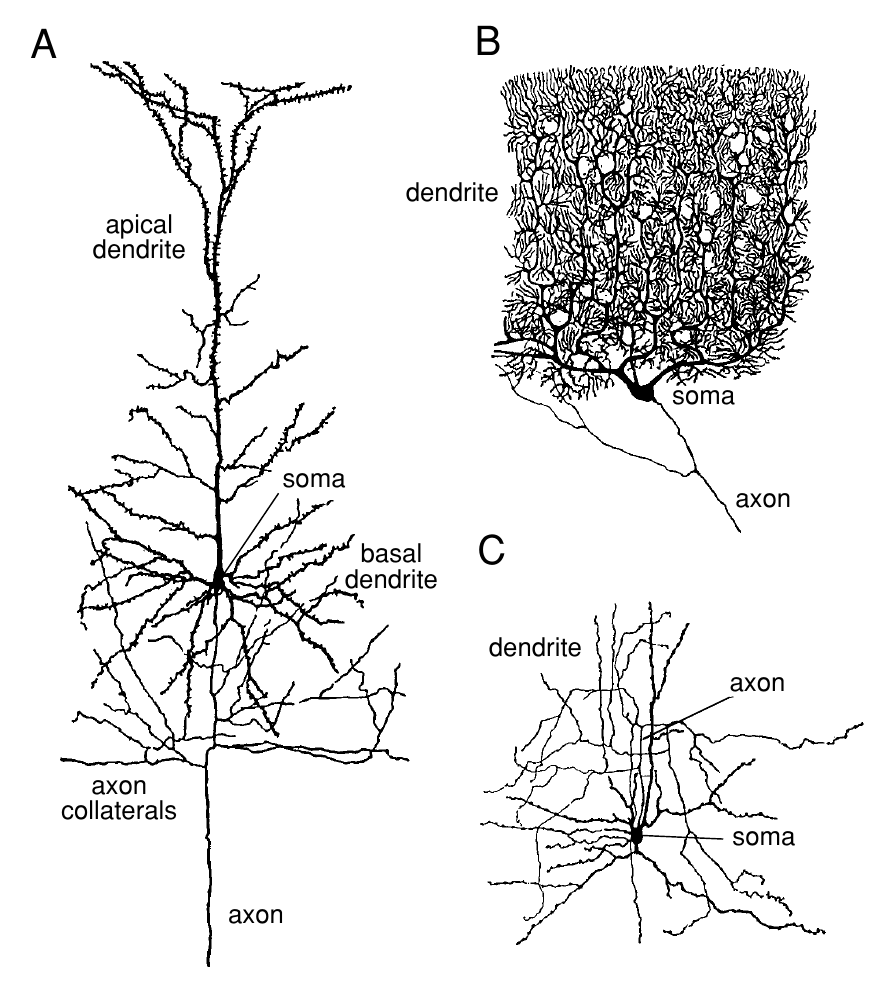
\includegraphics[width=0.62\linewidth]{neurons}}
\figcap{Three neurons drawn from real cells (lecture slide 4). (A) a cortical pyramidal cell with apical and basal
dendrites, soma, axon and axon collaterals; (B) a Purkinje cell of the cerebellum with its huge, dense dendritic fan;
(C) a stellate cell. The shapes are very different, but each has a soma, an axon and dendrites.}
\end{center}

\begin{intuition}[Why are neurons shaped like trees?]
To connect, the axon of one neuron must physically touch the dendrite of another. So a neuron that listens to many
others needs a big dendritic tree. The cerebellar Purkinje cell (B) receives input from \emph{hundreds of thousands}
of neurons, and its dendrites fill a huge fan. A cerebellar granule cell receives from about four neurons, and its
dendritic tree is tiny \src{LMLF 1.1.3}. \textbf{Shape follows the number of inputs.}
\end{intuition}

\subsection{The neuron's electricity: membrane potential, ion channels, ion pumps}\label{sec:elec}

The lecture says that ``the dynamics of the membrane potential are determined by the flow of ions through ion
channels and ion pumps''. Here is what each of these words means, following \src{LMLF 1.1.2}.

\begin{defn}[Ion]
An \term{ion} is an atom that carries an electric charge. Body fluids are salty water, full of ions. The two that matter most here are both positive:
\term{sodium} (Na$^+$) and \term{potassium} (K$^+$).
\end{defn}

\begin{defn}[Membrane]
The \term{membrane} is the thin fatty skin (a lipid bilayer) around the cell. Ions cannot pass through the fat itself, so the membrane separates two salty
liquids, the \emph{inside} and the \emph{outside} of the neuron.
\end{defn}

\begin{defn}[Ion pump]
An \term{ion pump} is a membrane protein that uses energy to push ions \emph{against} their natural flow. Pumps keep
K$^+$ concentrated \emph{inside} the cell and Na$^+$ concentrated \emph{outside}. They act like a battery charger:
they build up concentration differences that other proteins can later spend.
\end{defn}

\begin{defn}[Ion channel]
An \term{ion channel} is a pore-forming protein in the membrane. When it is open, it lets one specific kind of ion
through (a potassium channel passes K$^+$, a sodium channel passes Na$^+$). Ion channels are tiny, about $5$\,nm
(see the potassium channel in \S\ref{sec:scales}).
\end{defn}

\begin{defn}[Membrane potential]
The \term{membrane potential} $V$ is the voltage of the inside of the cell relative to the outside, measured in
millivolts (mV). At rest it is about $\hl{-70\,\text{mV}}$: the inside is negative.
\end{defn}

\textbf{Why is the inside negative?} Step by step:
\begin{enumerate}
  \item The pumps make K$^+$ more concentrated inside than outside.
  \item At rest, most of the open channels are \emph{potassium} channels.
  \item So K$^+$ ions leak \emph{out} along their concentration difference.
  \item Each K$^+$ that leaves carries a $+$ charge out, so the inside becomes negative.
  \item The result is a resting potential of about $-70$\,mV.
\end{enumerate}

\begin{defn}[Depolarize / hyperpolarize]
To \term{depolarize} means to make $V$ less negative (for example $-70\to-60$\,mV), which pushes the neuron towards firing.
To \term{hyperpolarize} means to make $V$ more negative (for example $-70\to-80$\,mV), which pushes it away from firing.
Na$^+$ flowing in depolarizes; K$^+$ flowing out hyperpolarizes.
\end{defn}

\section{Spikes (action potentials)}

\begin{defn}[Spike / action potential]
When the membrane potential reaches a \term{threshold}, a highly nonlinear process starts and lasts about
\hl{1\,ms}: the voltage shoots up and comes straight back down. This brief pulse is a \term{spike}, also called an
\term{action potential}. Spikes travel along the axon and provide input to the neuron's \term{postsynaptic partners}
(the neurons its axon connects to).
\end{defn}

\begin{center}
\begin{minipage}{0.3\linewidth}\centering
\fcolorbox{border}{white}{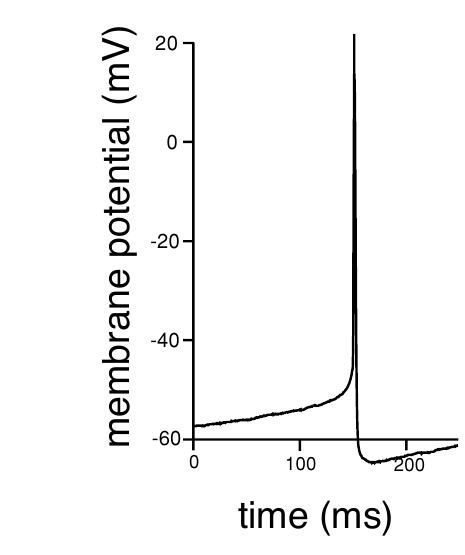
\includegraphics[width=\dimexpr\linewidth-7pt\relax]{spike_trace}}
\end{minipage}\hfill
\begin{minipage}{0.64\linewidth}
\figcap{A recorded spike (lecture slide 9). For $\sim$150\,ms the membrane potential creeps up slowly from about
$-57$\,mV. Once it crosses threshold it jumps to about $+20$\,mV and falls back in about 1\,ms, briefly overshooting
below where it started.}
\end{minipage}
\end{center}

\textbf{The mechanism, step by step} \src{LMLF 1.1.2}:
\begin{enumerate}
  \item Inputs depolarize the membrane a little.
  \item Sodium channels are \emph{voltage dependent}: depolarization opens some of them.
  \item Na$^+$ rushes in, which depolarizes the membrane further and opens even more sodium channels.
  \item Past the threshold (about $-50$\,mV) this \hl{positive feedback runs away}: $V$ rises to about $+40$\,mV in under a millisecond.
  \item The sodium channels then shut (inactivate) and extra potassium channels open. K$^+$ flows out and $V$ returns to rest.
\end{enumerate}

\begin{example}[Spike numbers]
Rest $-70$\,mV, threshold $\approx -50$\,mV, peak $\approx +40$\,mV. A single spike is therefore a swing of about
$110$\,mV in about $1$\,ms. The inputs that build up to it move $V$ by only a few mV each.
\end{example}

\begin{intuition}[Stereotyped, all-or-none]
Spikes have \hl{highly stereotyped temporal dynamics}: every spike of a neuron looks the same. Either the threshold is
crossed and a full spike happens, or it is not and nothing happens. Adrian showed in the 1920s that a stronger stimulus does \emph{not} make bigger spikes.
It makes \emph{more} spikes per second \src{LMLF 1.1.2}.
\end{intuition}

\begin{formula}[Central dogma of neuroscience]
\textbf{Spikes are the currency of communication in the brain.} The \emph{shape} of a spike carries no information.
Only \emph{whether} and \emph{when} spikes occur (and therefore how many per second) carries information.
\end{formula}

\section{Chemical synapses}

\begin{defn}[Synapse, presynaptic, postsynaptic]
A \term{synapse} is the contact point where the axon of one neuron meets (usually) a dendrite of another. The sending neuron (its axon side) is the
\term{presynaptic neuron}. The receiving neuron (its dendrite side) is the \term{postsynaptic neuron}. In a chemical
synapse the two are separated by a gap of about $30$\,nm \src{LMLF 1.1.3}.
\end{defn}

\begin{center}
\begin{minipage}[b]{0.28\linewidth}\centering
\fcolorbox{border}{white}{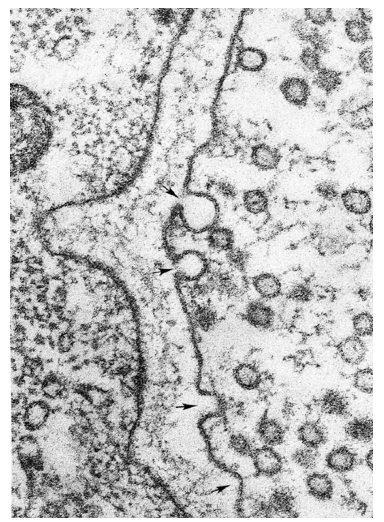
\includegraphics[width=\dimexpr\linewidth-7pt\relax]{synapse_em}}\\[-2pt]
{\scriptsize\color{muted}electron micrograph}
\end{minipage}\hspace{1.2em}
\begin{minipage}[b]{0.34\linewidth}\centering
\fcolorbox{border}{white}{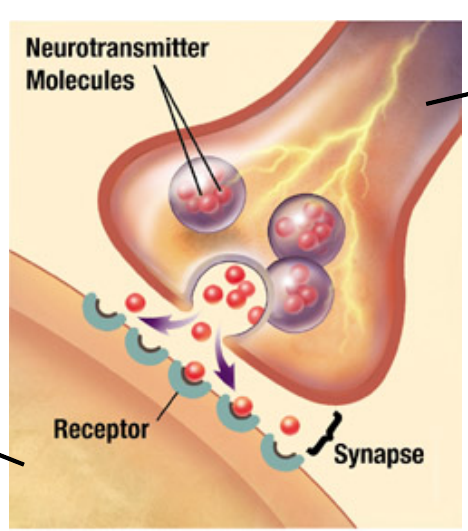
\includegraphics[width=\dimexpr\linewidth-7pt\relax]{synapse_diagram}}\\[-2pt]
{\scriptsize\color{muted}axon (top) onto dendrite (bottom)}
\end{minipage}
\figcap{Chemical synapses (lecture slide 10). Left: a real synapse under the electron microscope. The small round
vesicles hold neurotransmitter, and the arrows mark vesicles fusing with the membrane. Right: a cartoon of the same process.}
\end{center}

\textbf{What happens when a spike reaches a chemical synapse:}
\begin{enumerate}
  \item The spike arrives at the axon terminal of the presynaptic neuron.
  \item Small bubbles (\term{vesicles}) full of \term{neurotransmitter} molecules fuse with the membrane and release their contents into the gap.
  \item The neurotransmitter diffuses across the $\sim30$\,nm gap.
  \item It binds to \term{receptors}, proteins on the postsynaptic membrane.
  \item The receptors open or close ion channels. This \hl{converts the chemical signal back into an electrical signal}
        and changes the postsynaptic membrane potential.
\end{enumerate}

\begin{defn}[Excitatory and inhibitory synapses]
An \term{excitatory} synapse \emph{depolarizes} the postsynaptic neuron (moves it towards threshold). An
\term{inhibitory} synapse \emph{hyperpolarizes} it (moves it away from threshold).
\end{defn}

\begin{pitfall}[Slide wording]
The slide says synapses ``may either hyperpolarize or polarise the membrane potential''. The intended words are
\textbf{hyperpolarize (inhibit) or \emph{depolarize} (excite)}. The membrane is always polarized; a synapse makes it more or less so.
\end{pitfall}

\begin{formula}[Dale's principle]
\textbf{The synaptic connections \emph{from} a given neuron are either all excitatory or all inhibitory.}
A neuron releases the same neurotransmitters at all its terminals, so it has the same sign at every target.
Therefore we can label whole \emph{neurons} as \term{excitatory} or \term{inhibitory}.
\end{formula}

\begin{pitfall}[``From'', not ``to'']
Dale's principle concerns the \emph{outgoing} synapses. A neuron can \emph{receive} both excitatory and inhibitory
input; only what it \emph{sends} has one sign. In the rate model below this means that all the weights in one
\emph{column} $j$ of $J$ (the synapses out of neuron $j$) have the same sign. The weights in a row can have mixed signs.
\end{pitfall}

\section{The neuron as a computational unit: the rate model}

The lecture now strips the biology down to a simple computing element.

\begin{intuition}[Simple view of a neuron]
A neuron
\begin{enumerate}
  \item receives input in the form of spikes;
  \item \hl{sums these inputs linearly}, with weights that reflect the strength of each synapse;
  \item decides, based on this linear sum, when to produce a spike.
\end{enumerate}
We usually go one step further and suppose that the neuron decides only on a \hl{firing rate}, the number of spikes per second, and we ignore the exact spike times.
\end{intuition}

\begin{defn}[Firing rate]
The \term{firing rate} $r$ of a neuron is how many spikes it emits per second, in Hz. Example: 30 spikes in half a
second $\Rightarrow r = 60$\,Hz.
\end{defn}

\begin{center}
\fcolorbox{border}{white}{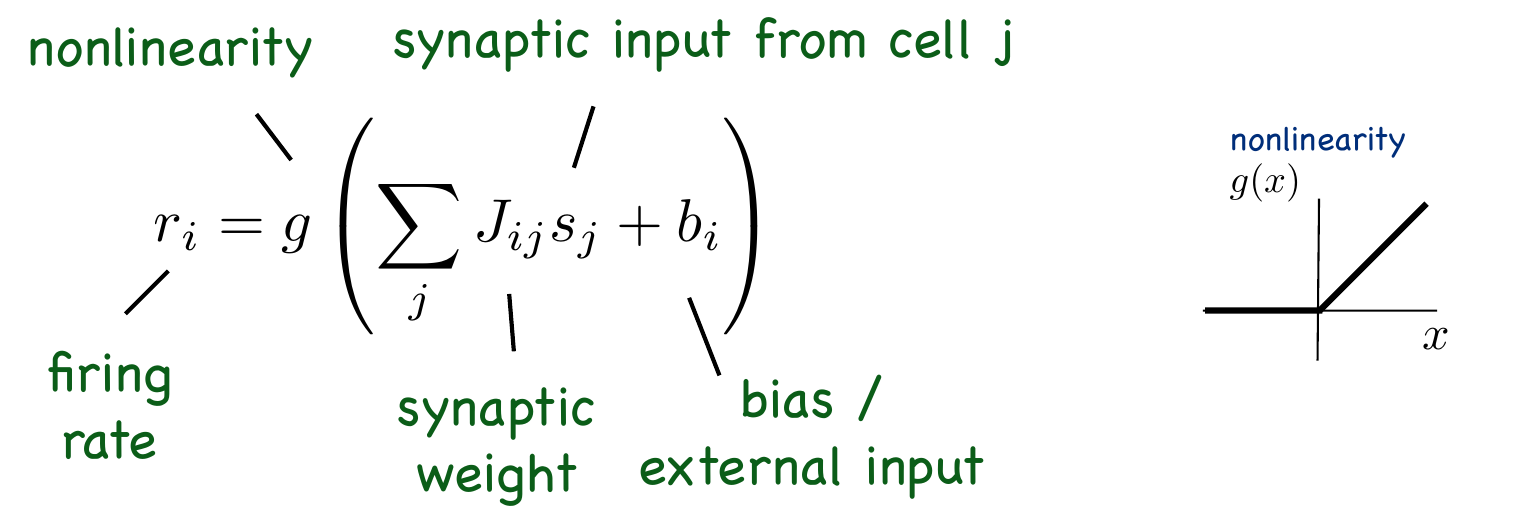
\includegraphics[width=0.82\linewidth]{rate_model_annotated}}
\figcap{The rate model as annotated in the lecture (slide 12), with the threshold-linear nonlinearity on the right.}
\end{center}

\begin{formula}[Rate model (no dynamics yet)]
\[
r_i = g\Big(\sum_j J_{ij}\, s_j + b_i\Big)
\quad\xrightarrow{\ s_j \,=\, r_j\ }\quad
r_i = g\Big(\sum_j J_{ij}\, r_j + b_i\Big)
\]
\begin{tabular}{@{}ll@{}}
$r_i$ & firing rate of neuron $i$\\
$s_j$ & synaptic input from cell $j$\\
$J_{ij}$ & \term{synaptic weight} from neuron $j$ \emph{to} neuron $i$ ($>0$ excitatory, $<0$ inhibitory)\\
$b_i$ & bias / external input to neuron $i$\\
$g$ & the \term{nonlinearity} (activation function)
\end{tabular}
\end{formula}

\begin{pitfall}[Index order]
$J_{ij}$ is the synapse \textbf{from $j$ to $i$}: the first index is the receiver. Row $i$ of $J$ lists everything neuron $i$ hears.
\end{pitfall}

\begin{defn}[Nonlinearity $g$]
$g$ turns the total input $h$ into a firing rate. The lecture draws the \term{threshold-linear} function (also called ReLU):
\[ g(x) = \lfloor x\rfloor = \begin{cases} x, & x>0\\ 0, & x\le 0.\end{cases} \]
It encodes the fact that \hl{a firing rate cannot be negative}: below threshold the neuron is silent, above it the rate
grows with the input. Other common choices in the book are the S-shaped \emph{logistic} function, which also saturates, and,
for small changes, the linear function $g(x)=x$ \src{LMLF 2.2.1}.
\end{defn}

\begin{example}[Three neurons, one step]
Neuron 3 receives from neurons 1 and 2. Take $r_1 = 10$\,Hz, $r_2 = 20$\,Hz, $J_{31}=0.5$ (excitatory),
$J_{32}=-0.4$ (inhibitory), bias $b_3=2$, and $g$ threshold-linear.
\[ h_3 = 0.5\cdot 10 + (-0.4)\cdot 20 + 2 = 5 - 8 + 2 = -1 \;\Rightarrow\; r_3 = g(-1) = 0\ \text{Hz}. \]
If neuron 2 slows to $r_2=5$\,Hz: $h_3 = 5 - 2 + 2 = 5 \Rightarrow r_3 = 5$\,Hz. Inhibition switched the neuron
off, and removing most of it switched the neuron back on.
\end{example}

\begin{intuition}[Identifying $s_j$ with $r_j$]
The input neuron $i$ gets from cell $j$ is assumed to be proportional to how fast $j$ fires. Once $s_j=r_j$, the same
rates appear on both sides of the equation: every neuron's output is somebody else's input. That is what
makes it a \emph{network}.
\end{intuition}

\begin{pitfall}[No dynamics yet]
The lecture stresses: \textbf{so far there are no dynamics}. The equation says what the rate \emph{is}, not how it \emph{changes in time}.
Time enters in the bonus hour and the TA session as $\tau\dot r_i = -r_i + g\big(\sum_j J_{ij}r_j + b_i\big)$ (Part B, \S\ref{sec:tie}).
\end{pitfall}

\section{Scales in the human brain}\label{sec:scales}

\subsection{Length}

The brain has structure on every length scale, from single molecules to the whole nervous system.

\begin{center}
\fcolorbox{border}{white}{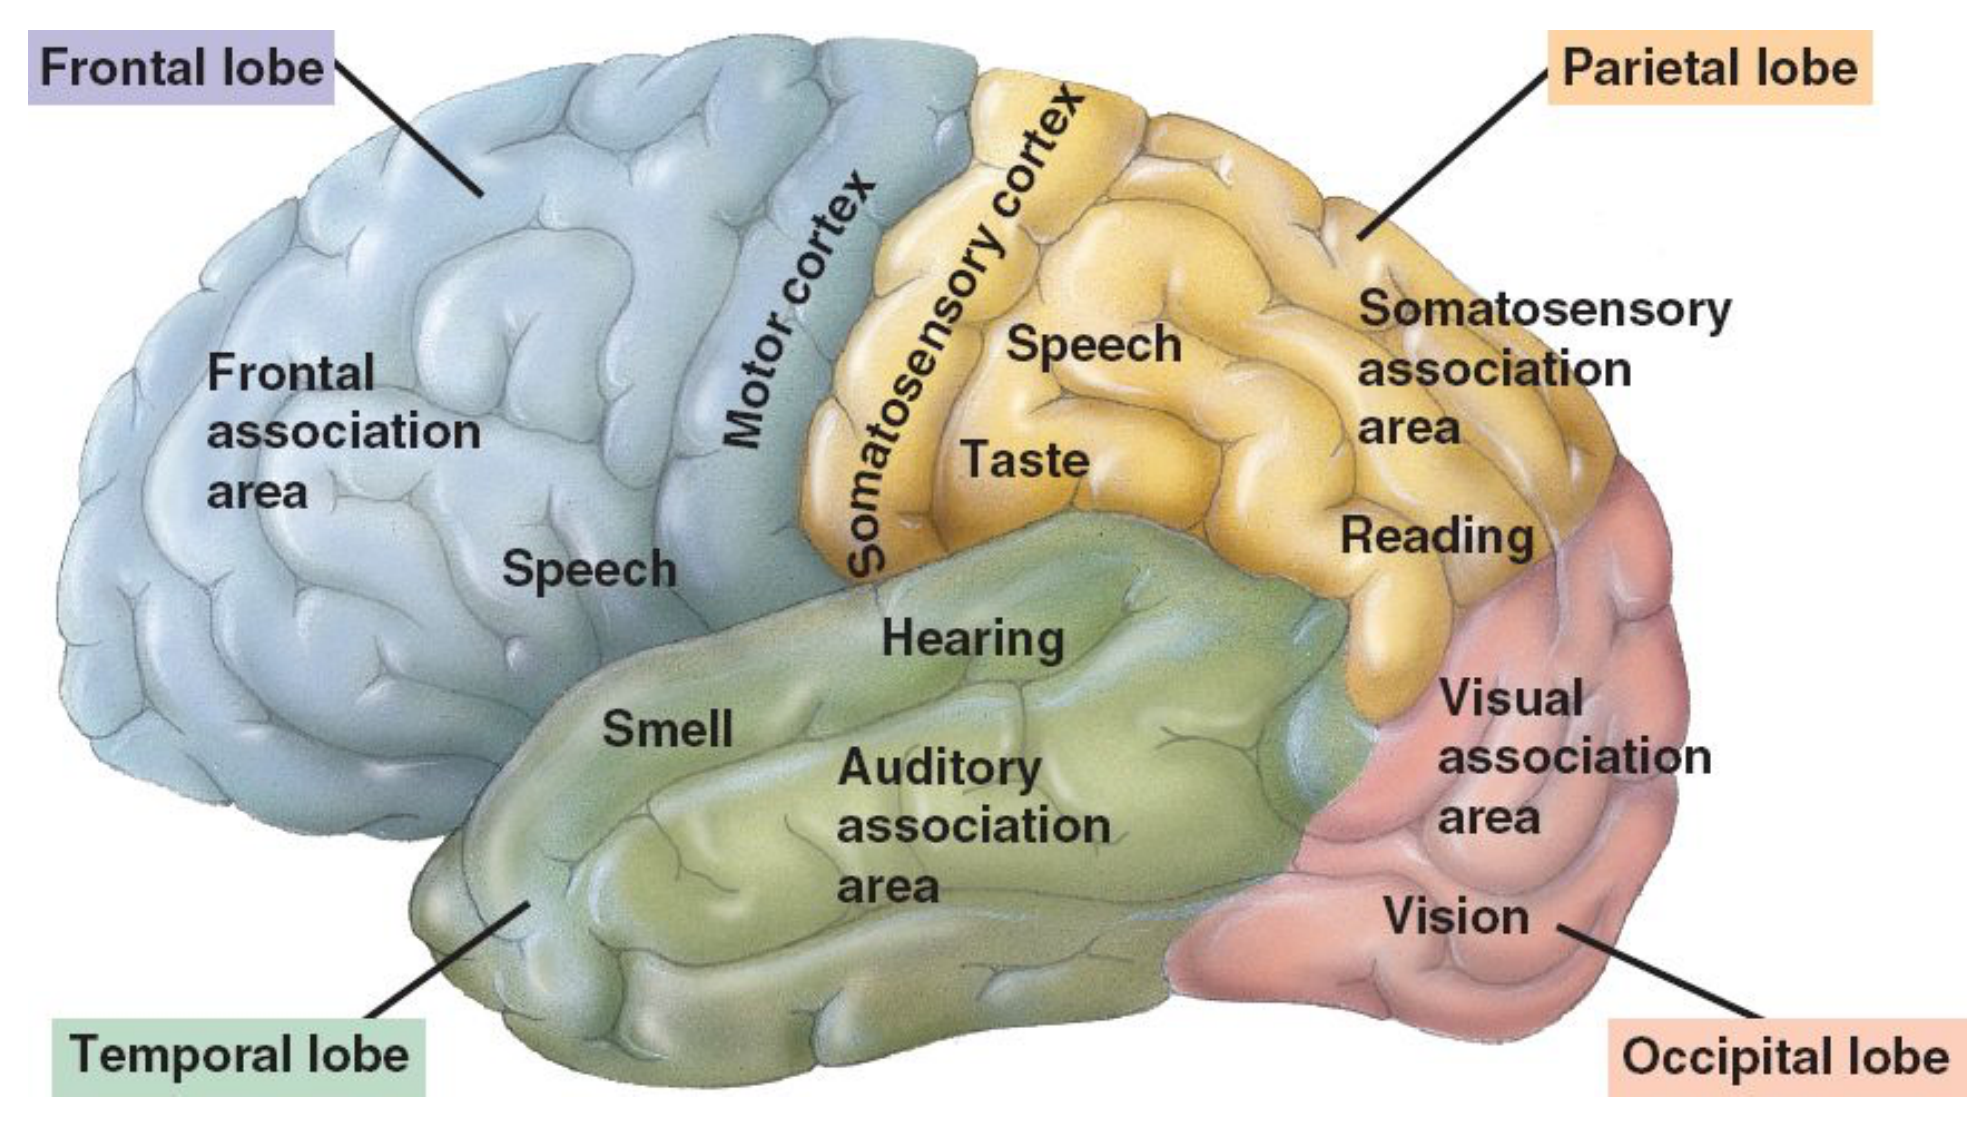
\includegraphics[width=0.72\linewidth]{cortex_lobes}}
\figcap{The \term{cerebral cortex} (Hebrew: \emph{klipat ha-moach}, ``the brain's peel''), the folded outer sheet of the
brain (slide 14). It is divided into lobes: frontal (motor cortex, speech, association areas), parietal (somatosensory,
reading), temporal (hearing, smell) and occipital (vision).}
\end{center}

\begin{center}
\renewcommand{\arraystretch}{1.25}
\begin{tabular}{>{\columncolor{border}}l l L{7.4cm}}
\thd{LEVEL} & \cellcolor{border}\thd{SIZE} & \cellcolor{border}\thd{WHAT IT IS}\\
\rowcolor{surface} \cellcolor{border}\color{surface}Molecules & 1\,nm & single proteins, e.g.\ an ion channel ($\sim$5\,nm)\\
\rowcolor{surface2} \cellcolor{border}\color{surface}Synapses & 1\,$\mu$m & one axon--dendrite contact\\
\rowcolor{surface} \cellcolor{border}\color{surface}Neurons & 10--100\,$\mu$m & size of the cell body\\
\rowcolor{surface2} \cellcolor{border}\color{surface}Local networks & 1\,mm & a cortical column, $\sim10^4$ neurons\\
\rowcolor{surface} \cellcolor{border}\color{surface}Maps & 1\,cm & an area representing e.g.\ the visual field or body surface\\
\rowcolor{surface2} \cellcolor{border}\color{surface}Systems & 10\,cm & e.g.\ the visual system, the motor system\\
\rowcolor{surface} \cellcolor{border}\color{surface}Central nervous system & 1\,m & brain + spinal cord\\
\end{tabular}
\end{center}

\begin{center}
\begin{minipage}[b]{0.4\linewidth}\centering
\fcolorbox{border}{white}{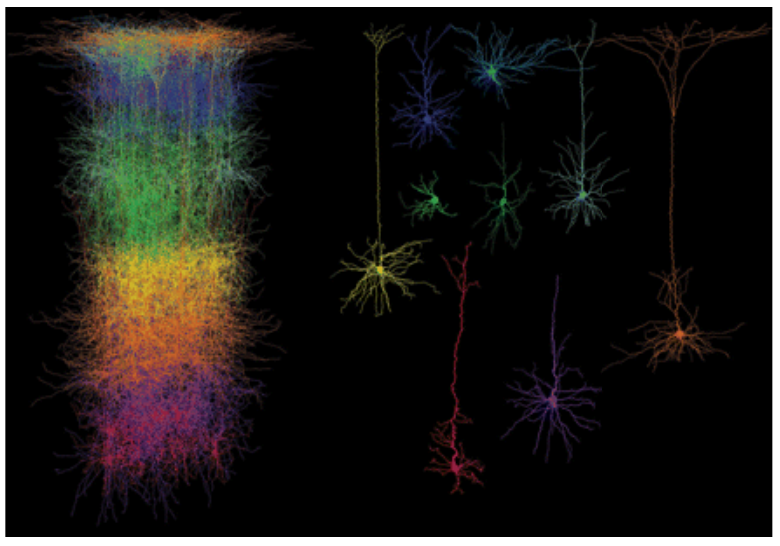
\includegraphics[width=\dimexpr\linewidth-7pt\relax]{cortical_column}}\\[-2pt]
{\scriptsize\color{muted}cortical column, $\sim$1\,mm (Oberlaender \dots\ Sakmann 2011)}
\end{minipage}\hfill
\begin{minipage}[b]{0.27\linewidth}\centering
\fcolorbox{border}{white}{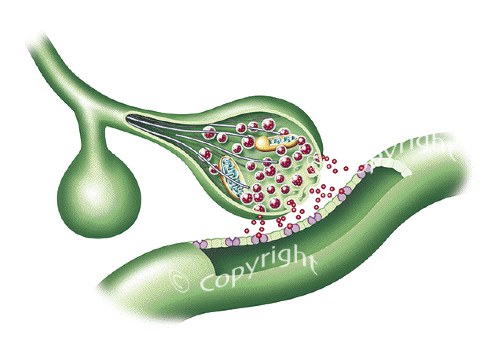
\includegraphics[width=\dimexpr\linewidth-7pt\relax]{synapse_3d}}\\[-2pt]
{\scriptsize\color{muted}synapse, $\sim$1\,$\mu$m}
\end{minipage}\hfill
\begin{minipage}[b]{0.27\linewidth}\centering
\fcolorbox{border}{white}{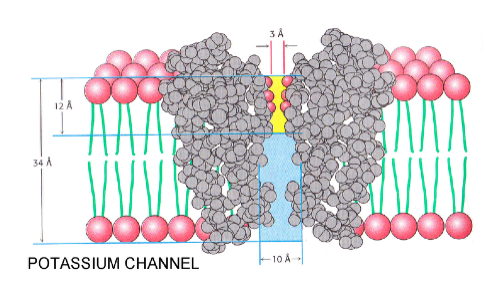
\includegraphics[width=\dimexpr\linewidth-7pt\relax]{ion_channel}}\\[-2pt]
{\scriptsize\color{muted}potassium channel, $\sim$5\,nm}
\end{minipage}
\figcap{Three of the length scales (slide 16). In the column the colours mark neurons whose cell bodies sit in different layers.}
\end{center}

\begin{intuition}[Where this course lives]
The lecture circles two levels: \hl{local networks (1\,mm)} and \hl{maps (1\,cm)}. The rate model describes
networks of many neurons. It does not describe molecules or the inside of a single synapse.
\end{intuition}

\subsection{Time}

\begin{center}
\renewcommand{\arraystretch}{1.25}
\begin{tabular}{>{\columncolor{border}}l l L{6.2cm}}
\thd{PROCESS} & \cellcolor{border}\thd{TIME} & \cellcolor{border}\thd{MEANING}\\
\rowcolor{surface} \cellcolor{border}\color{surface}Action potential & 1\,ms & duration of one spike\\
\rowcolor{surface2} \cellcolor{border}\color{surface}Membrane integration time & 10\,ms & how long the membrane ``remembers'' input\\
\rowcolor{surface} \cellcolor{border}\color{surface}Synaptic integration time & 1--100\,ms & how long one synaptic input lasts\\
\rowcolor{surface2} \cellcolor{border}\color{surface}Short-term synaptic plasticity & 0.1--1\,s & synapses temporarily strengthen/weaken with use\\
\rowcolor{surface} \cellcolor{border}\color{surface}Long-term synaptic plasticity & 1--$10^4$\,s & lasting change of synaptic strength\\
\rowcolor{surface2} \cellcolor{border}\color{surface}Long-term structural changes & $10^6$--$10^9$\,s & long-term memory, learning\\
\end{tabular}
\end{center}

\begin{example}[How wide is the range?]
From $10^{-3}$\,s (a spike) to $10^{9}$\,s ($\approx 30$ years) is a factor of $10^{12}$. Lengths run from $10^{-9}$\,m to $1$\,m,
a factor of $10^{9}$. The membrane integration time of $\sim10$\,ms is the $\tau$ that appears in the rate model
(Part B, \S\ref{sec:tie}).
\end{example}

\section{Numbers in human and non-human brains}

\begin{center}
\renewcommand{\arraystretch}{1.25}
\begin{tabular}{>{\columncolor{border}}l c c c}
\thd{ANIMAL} & \cellcolor{border}\thd{\# NEURONS} & \cellcolor{border}\thd{\# SYNAPSES} & \cellcolor{border}\thd{SYNAPSES / NEURON}\\
\rowcolor{surface} \cellcolor{border}\color{surface}\emph{C.\ elegans} (worm) & 302 & 5000 & $\approx 17$\\
\rowcolor{surface2} \cellcolor{border}\color{surface}\emph{Drosophila} (fruit fly) & $10^5$ & $10^7$ & $10^2$\\
\rowcolor{surface} \cellcolor{border}\color{surface}\emph{M.\ musculus} (mouse) & $10^8$ & $10^{11}$ & $10^3$\\
\rowcolor{surface2} \cellcolor{border}\color{surface}\emph{H.\ sapiens} (human) & $10^{11}$ & $10^{14}$--$10^{15}$ & $10^3$--$10^4$\\
\rowcolor{surface} \cellcolor{border}\color{surface}Human cortex & $2\times10^{10}$ & & \\
\rowcolor{surface2} \cellcolor{border}\color{surface}One cortical column (1\,mm$\times$1\,mm) & $10^4$ & $10^7$--$10^8$ & $10^3$--$10^4$\\
\end{tabular}
\end{center}

\begin{example}[Reading the table]
The last column is just synapses $\div$ neurons. For a human: $10^{14}/10^{11} = 10^3$ up to $10^{15}/10^{11}=10^4$. So
a typical neuron \hl{listens to thousands of others}. A single column already holds as many synapses as an entire fly brain.
\end{example}

\section{Why the brain is hard: challenges}

\begin{itemize}
  \item \textbf{Collective dynamics of many computational units.} Behaviour emerges from $10^{11}$ interacting neurons, not from any single one.
  \item \textbf{A vast range of temporal and spatial scales} (\S\ref{sec:scales}).
  \item \textbf{Complex structure on all scales, most of it unknown.} Which details are important? At what level of description should we model?
  \item \textbf{Function}: the brain computes and processes information. Understanding it means understanding \emph{what} it computes.
  \item \textbf{Evolution was free to tweak properties on all scales} to achieve a function, and it often uses multiple mechanisms for the same job.
\end{itemize}

\section{Computational neuroscience}

\begin{defn}[Computational neuroscience]
\term{Computational neuroscience} (Hebrew: \emph{chishuviyut atzabit}) is the study of the brain in terms of the
\hl{computational and informational properties} of the nervous system. The interest is often at the \term{systems level}:
the collective behaviour of many neurons.
\end{defn}

\textbf{Computations the brain performs:} sensory perception (discrimination, object recognition, \dots), decision
making, generation of motor output, memory, learning, language and creativity.

\begin{intuition}[Information everywhere]
Information plays a central role in all of these: it is \hl{represented (coded), extracted, discarded, relayed and stored}.
The ``coding'' half of the course title is about this.
\end{intuition}

\section{New tools in neuroscience}

\begin{center}
\begin{minipage}[c]{0.3\linewidth}\centering
\fcolorbox{border}{white}{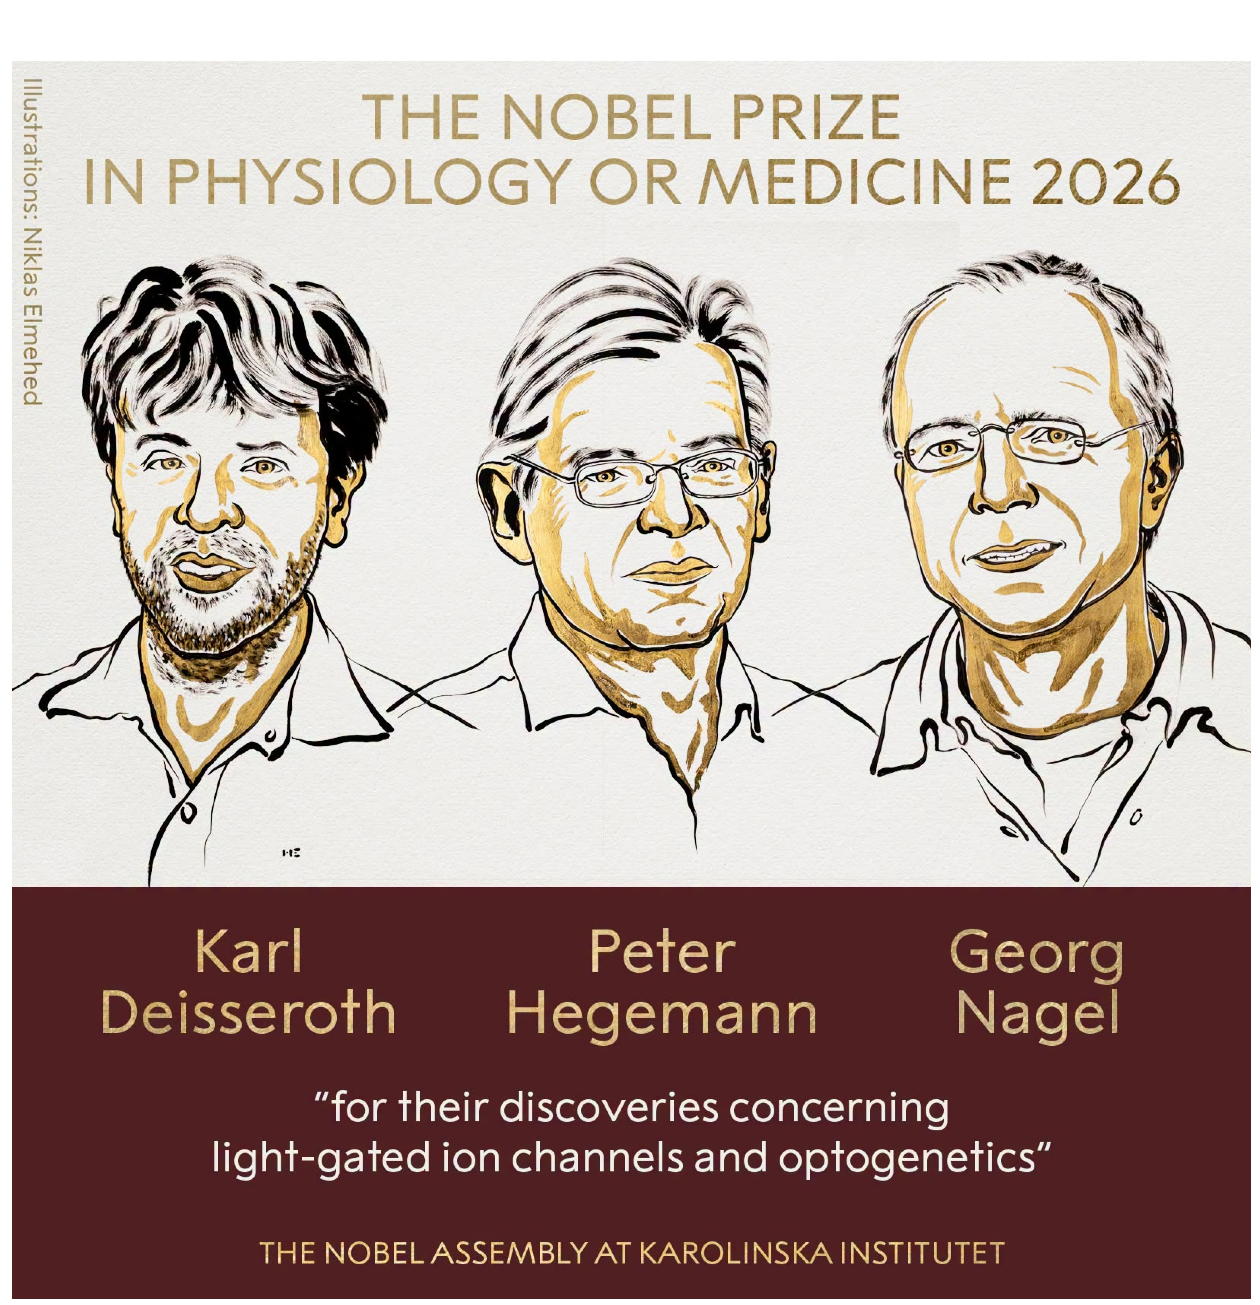
\includegraphics[width=\dimexpr\linewidth-7pt\relax]{nobel_optogenetics}}
\end{minipage}\hfill
\begin{minipage}[c]{0.16\linewidth}\centering
\fcolorbox{border}{white}{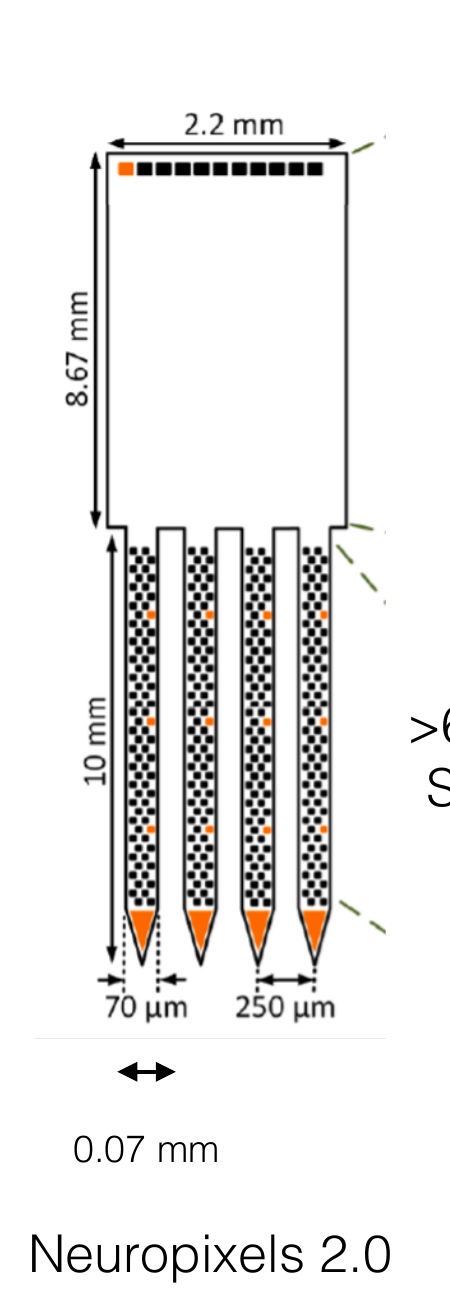
\includegraphics[width=\dimexpr\linewidth-7pt\relax]{neuropixels}}
\end{minipage}\hfill
\begin{minipage}[c]{0.48\linewidth}
\figcap{Left: the 2026 Nobel Prize in Physiology or Medicine (Deisseroth, Hegemann, Nagel) for light-gated ion channels
and optogenetics (slide 23). Right: a Neuropixels 2.0 probe, four shanks 70\,$\mu$m wide with more than 6000 recording sites (slide 24).}
\end{minipage}
\end{center}

\begin{defn}[Optogenetics]
\term{Optogenetics}: neurons are genetically made to produce \emph{light-gated ion channels}, i.e.\ ion channels (\S\ref{sec:elec})
that open when light shines on them. Shining light then \hl{activates or silences chosen neurons}. Because a light-opened
Na$^+$-type channel depolarizes and a Cl$^-$/K$^+$-type one hyperpolarizes, the same trick works in both directions.
\end{defn}

\begin{defn}[Calcium imaging]
\term{Calcium imaging}: neurons are made to express a molecule that glows when it binds calcium. Spikes are followed by
calcium entry, so the brightness of a neuron is a proxy for its activity. This gives the firing \emph{rates} of many neurons, but
not the individual spikes \src{LMLF 2.2.3}.
\end{defn}

The lecture lists the technological revolutions:
\begin{itemize}
  \item optogenetic activation or silencing of individual neurons;
  \item simultaneous recordings from hundreds of neurons (silicon probes, calcium imaging);
  \item all of this in awake, freely behaving animals, relying heavily on genetic tools;
  \item anatomical tracing of connectivity (\term{connectomics}).
\end{itemize}

\begin{intuition}[Why this favours the rate model]
Calcium imaging reports roughly how active each neuron is, not when each spike happened. The rate model is
the simplest dynamical model whose variables are exactly what these experiments measure \src{LMLF 2.2.3}.
\end{intuition}

\section{A case study: heading in the fruit fly brain}

\begin{center}
\fcolorbox{border}{white}{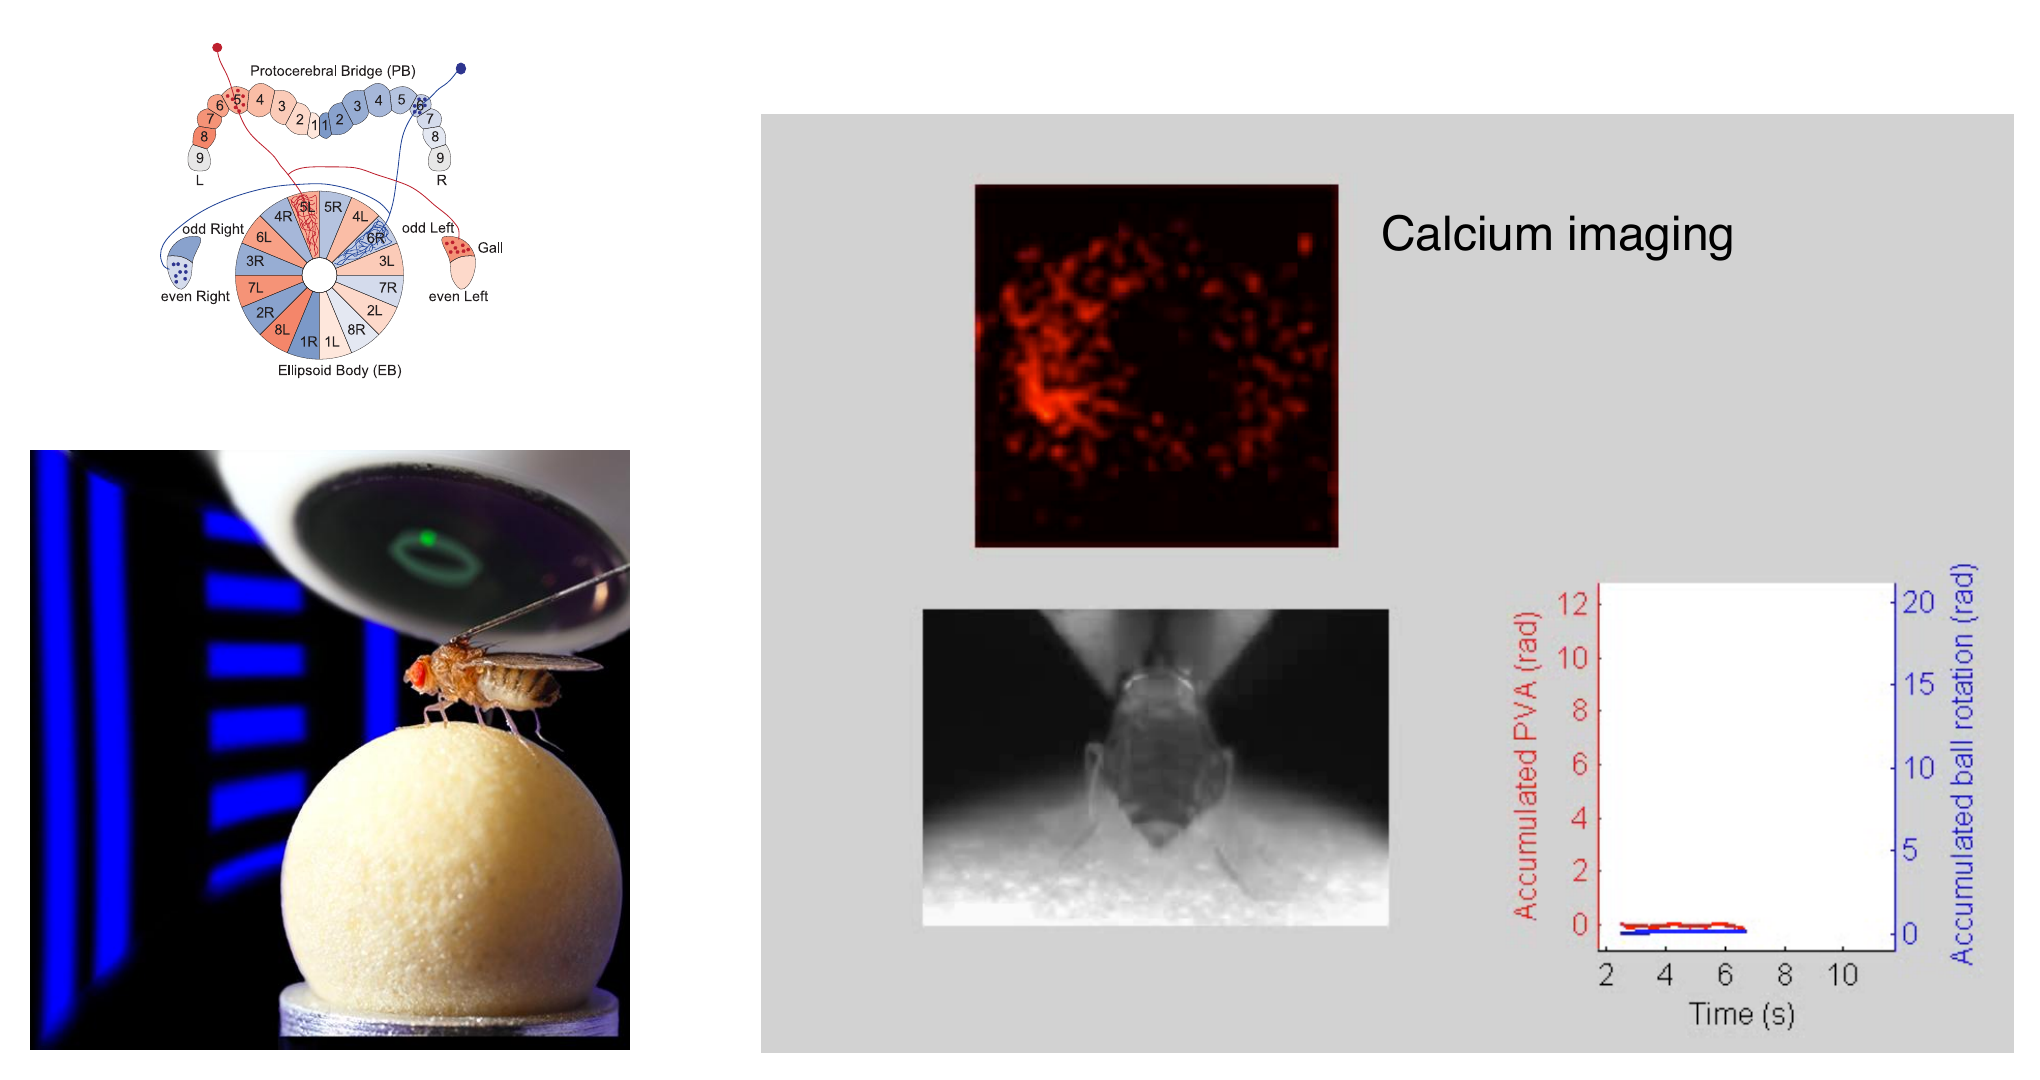
\includegraphics[width=0.9\linewidth]{fly_heading_setup}}
\figcap{Representation of heading in the fruit fly (slide 25; Seelig \& Jayaraman, Nature 2015; Kim, Rouault, Druckmann \&
Jayaraman, Science 2017). Bottom left: a fly walks on an air-supported ball in front of a visual display while a microscope records from its brain.
Top left: the \term{ellipsoid body (EB)}, a ring of 16 wedges. Right: calcium imaging of the ring and the fly's turns on the ball.}
\end{center}

\begin{center}
\fcolorbox{border}{white}{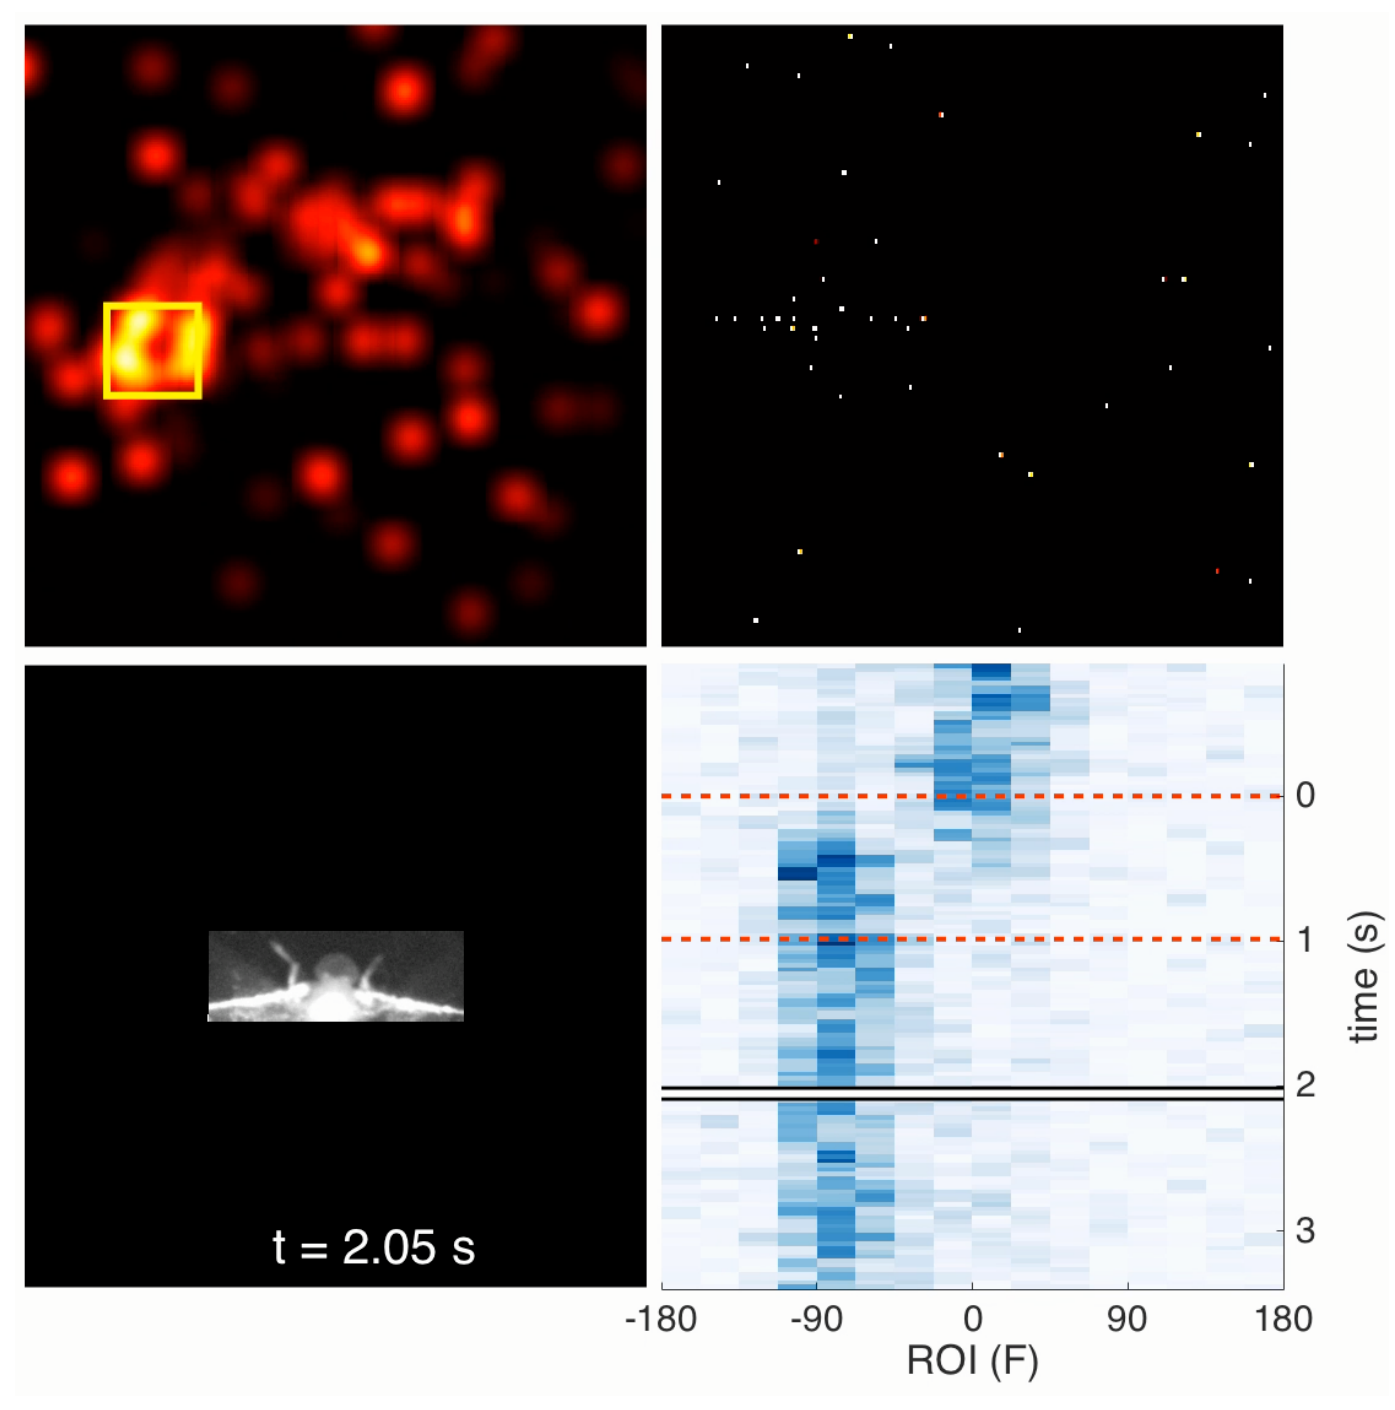
\includegraphics[width=0.55\linewidth]{fly_heading_bump}}
\figcap{Slide 26. Bottom right: activity of each wedge of the ring (x-axis, from $-180^\circ$ to $180^\circ$) over time (y-axis). At any moment
only a few neighbouring wedges are active, forming a \term{bump}. The bump moves around the ring as the fly turns, and it stays
in place when the fly stands still, even in the dark.}
\end{center}

\begin{intuition}[What the experiment shows]
The ring of neurons works like an \hl{internal compass}. The position of the activity bump on the ring \emph{is} the fly's
heading. When the fly turns, the bump moves by the same angle. The bump persists without visual input, so the network \emph{remembers} the heading.
\end{intuition}

\section{The theoretical questions: dynamics and coding}

The fly compass raises the two families of questions that give the course its name:

\begin{plainbox}
\textbf{\textcolor{ppink}{Dynamics}}
\begin{itemize}
  \item How can a network of neurons generate activity structured as a bump?
  \item How can memory be sustained in the ongoing neural activity?
  \item How does the network respond to inputs? (``input selectivity'')
\end{itemize}
\textbf{\textcolor{ppink}{Coding}}
\begin{itemize}
  \item What is the best way to decode the represented heading from the spikes of these neurons?
  \item How precise is the neural representation?
\end{itemize}
\end{plainbox}

\section{Learning}

The word ``learning'' is used in two ways in neuroscience:
\begin{defn}[Learning, two views]
\begin{itemize}
  \item \textbf{Mechanistic}: any process that involves long-term changes in synaptic connectivity in the brain
        (\term{synaptic plasticity}). In the rate model, this means changes of the weights $J_{ij}$.
  \item \textbf{Functional}: shaping neural connectivity to \emph{achieve a function}. An important distinction here is
        \term{supervised} learning (a teacher signal says what the right output is) versus \term{unsupervised} learning (no teacher).
\end{itemize}
\end{defn}
Learning is covered in a separate course (\emph{Neural Learning}, semester B), not in this one.

\section{Roadmap of the course}

\begin{center}
\renewcommand{\arraystretch}{1.2}
\begin{tabular}{L{7.2cm} L{7.2cm}}
\rowcolor{border}\thd{PART I: NEURAL NETWORK DYNAMICS (LOEWENSTEIN)} & \thd{PART II: NEURAL CODING (BURAK)}\\
\rowcolor{surface}
\textbf{Rate model} (ch.\ 2): single neuron, network dynamics; autapse, mutual inhibition, oscillations.\newline
\textbf{Feature selectivity} (ch.\ 3): feedforward and recurrent networks, ring model, amplification.\newline
\textbf{Working memory} (ch.\ 4): line attractor, integration, ring model.\newline
\textbf{Balanced networks} (ch.\ 6).\newline
\emph{Tools: linear algebra, differential equations.}
&
\textbf{Decoders}: maximum-likelihood and MAP decoders, discriminators, estimators (Fisher information, Cram\'er--Rao bound), Poisson neurons.\newline
\textbf{Efficient coding}: Shannon information, optimal nonlinearity, PCA, receptive fields in the retina.\newline
\emph{Tools: statistics, linear algebra.}
\end{tabular}
\end{center}
Part B and Part C below supply exactly the two Part I tools: differential equations and linear algebra.

% =================================================================
\parttitle{PART B \textperiodcentered\ BONUS HOUR 1}{Differential Equations: $\dot n = an$ and Its Relatives}
% =================================================================

\section{Why ``dynamics''?}

``Dynamic'' means \emph{characterized by constant change, activity or progress}. This course studies quantities that
keep changing, such as firing rates, and it cares more about \hl{how they change} than about the values they hold at any one moment.

\begin{intuition}[One path vs.\ all paths]
Knowing one trajectory of a system, out of infinitely many, tells you almost nothing. Understanding how \emph{all} the
trajectories behave tells you everything. \textbf{A dynamical system} is a set of differential equations used as a model of how something in the world changes.
\end{intuition}

\section{Vocabulary}

\begin{defn}[Derivative, dot notation]
$\dfrac{dn}{dt}$ is the rate of change of $n$ at time $t$. We also write it $\dot n(t)$ or simply $\dot n$ (Newton's dot notation).
Example: if $n$ goes from $100$ to $103$ in $0.1$ days, then $\dot n \approx 3/0.1 = 30$ per day.
\end{defn}

\begin{defn}[Differential equation]
A \term{differential equation} is an equation that relates an unknown \emph{function} to its derivative, for example $\dot n(t) = a\,n(t)$.
It is \term{first order} if only the first derivative appears, and \term{linear} if $n$ and $\dot n$ appear only to the first
power, without products \src{LMLF 2.A.1}.
\end{defn}

\begin{pitfall}[The unknown is a function, not a number]
Compare $f(x)=ax$ with $\dot n(t)=an(t)$. Solving for $x$ gives \emph{one number}. Solving the differential equation gives a
\emph{whole function} $n(t)$, i.e.\ a value at every time.
\end{pitfall}

\begin{defn}[Initial condition]
The \term{initial condition} $n(0)=n_0$ is the value at the start. A differential equation has a whole family of solutions,
and the initial condition picks out one of them.
\end{defn}

\section{A model of an epidemic}

The bonus hour builds an equation from a story. A mysterious illness spreads; you know roughly how many people get sick
and how many recover each day. Let $n(t)$ be the number of sick people at time $t$.

\begin{formula}[Epidemic model]
\[ \tau\,\frac{dn}{dt} = \tau\dot n(t) = \beta\, n(t) - \gamma\, n(t) \]
\begin{tabular}{@{}ll@{}}
$\beta n(t)$ & new infections: more sick people $\Rightarrow$ more infections ($\beta$ = rate of infection)\\
$-\gamma n(t)$ & recoveries: a fixed fraction $\gamma$ of the sick recover per unit time\\
$\tau$ & the \term{time constant}: the time frame of these processes (e.g.\ days)
\end{tabular}
\end{formula}

\textbf{Simplify.} Collect the terms and divide by $\tau$:
\[ \tau\dot n = (\beta-\gamma)\,n \;\iff\; \dot n = \underbrace{\frac{\beta-\gamma}{\tau}}_{a}\,n \;\iff\; \boxed{\ \dot n(t) = a\,n(t)\ } \]
The sign of $a$ tells the story:
\begin{itemize}
  \item $a>0$ ($\beta>\gamma$): more people get sick than recover, so $n$ grows.
  \item $a<0$ ($\beta<\gamma$): more people recover than get sick, so $n$ shrinks.
  \item $n(t_0)=0$: nobody is sick, so nobody infects or recovers, $\dot n=0$, and $n$ stays $0$ forever.
\end{itemize}

\section{Solving $\dot n = an$ step by step}

The trick is to multiply by a cleverly chosen function so that the left-hand side becomes one single derivative.

\textbf{Step 0: the product rule.}
\[ \frac{d}{dt}\big(f(t)\,g(t)\big) = \dot f(t)\,g(t) + f(t)\,\dot g(t). \]

\textbf{Step 1: move everything to one side.} $\dot n - a n = 0$.

\textbf{Step 2: multiply by $e^{-at}$.} $\dot n\, e^{-at} - a\,n\, e^{-at} = 0$.

\textbf{Step 3: recognise a product rule.} Take $f=n$ and $g=e^{-at}$, so $\dot g = -a e^{-at}$. Then
\[ \frac{d}{dt}\big(n\,e^{-at}\big) = \dot n\, e^{-at} + n\,(-a e^{-at}) = \dot n\, e^{-at} - a\,n\, e^{-at}, \]
which is exactly the left-hand side of Step 2. So
\[ \frac{d}{dt}\big(n(t)\,e^{-at}\big) = 0. \]

\textbf{Step 4: integrate.} A function whose derivative is $0$ is a constant: $n(t)\,e^{-at} = C$.

\textbf{Step 5: solve for $n$.} $n(t) = C e^{at}$.

\textbf{Step 6: name the constant.} At $t=0$: $n(0) = Ce^{0} = C$. So $C=n_0$:

\begin{formula}[Solution]
\[ \dot n = an,\quad n(0)=n_0 \qquad\Longrightarrow\qquad \boxed{\,n(t) = n_0\,e^{at}\,} \]
\end{formula}

\textbf{Check by plugging in.} $\dfrac{d}{dt}\big(n_0e^{at}\big) = a\,n_0e^{at} = a\,n(t)$. \checkmark

\begin{example}[Numbers for the epidemic]
Start with $n_0 = 100$ sick people, time in days.
\begin{center}
\renewcommand{\arraystretch}{1.2}
\begin{tabular}{>{\columncolor{border}}c c c}
\thd{DAY $t$} & \cellcolor{border}\thd{$a=+0.1$: $100e^{0.1t}$} & \cellcolor{border}\thd{$a=-0.1$: $100e^{-0.1t}$}\\
\rowcolor{surface} \cellcolor{border}\color{surface}0 & 100 & 100\\
\rowcolor{surface2} \cellcolor{border}\color{surface}7 & 201 & 49.7\\
\rowcolor{surface} \cellcolor{border}\color{surface}14 & 406 & 24.7\\
\rowcolor{surface2} \cellcolor{border}\color{surface}21 & 817 & 12.2\\
\rowcolor{surface} \cellcolor{border}\color{surface}30 & 2009 & 5.0\\
\end{tabular}
\end{center}
With $a=0.1$ the number \hl{doubles every $\ln 2/a \approx 6.9$ days}. With $a=-0.1$ it halves every $6.9$ days. Same speed,
opposite directions.
\end{example}

\begin{center}
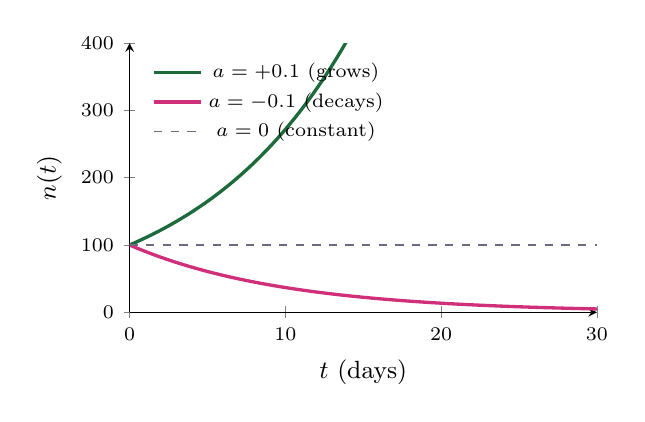
\begin{tikzpicture}
\begin{axis}[width=0.62\linewidth,height=5cm,xmin=0,xmax=30,ymin=0,ymax=400,
  xlabel={$t$ (days)},ylabel={$n(t)$},axis lines=left,tick label style={font=\scriptsize},
  label style={font=\small},legend style={font=\scriptsize,draw=none,fill=none},legend pos=north west]
  \addplot[pgreen,very thick,domain=0:30,samples=80]{100*exp(0.1*x)};
  \addplot[ppink,very thick,domain=0:30,samples=80]{100*exp(-0.1*x)};
  \addplot[muted,dashed,domain=0:30]{100};
  \legend{$a=+0.1$ (grows),$a=-0.1$ (decays),$a=0$ (constant)}
\end{axis}
\end{tikzpicture}
\figcap{$n(t)=n_0e^{at}$ for three values of $a$. The sign of $a$ alone decides between growth and decay.}
\end{center}

\begin{pitfall}[Limits of the model]
Every model is imperfect. This one:
\begin{enumerate}
  \item assumes an \textbf{infinite population}: with $a>0$, $n$ grows forever (on day 100 we would have $100e^{10}\approx 2.2$ million sick);
  \item is \textbf{continuous}: $n$ need not be an integer (3.1 sick people), and with $a<0$ it never reaches exactly $0$, it only approaches it.
\end{enumerate}
\end{pitfall}

\section{When we cannot solve: three other ways to analyse}

Most equations in the course cannot be solved by a formula. The bonus hour names three alternatives:

\begin{enumerate}
  \item \textbf{Numerical methods.} Use the derivative to step forward in time on a computer. The simplest is the
        \term{Euler method} \src{LMLF 2.A.1}: $n(t+dt) \approx n(t) + \dot n(t)\,dt$.
  \item \textbf{Fixed points.} Ask questions about the derivative instead of the function.
  \item \textbf{Geometry.} Use the sign of the derivative: $\dot n>0$ means $n$ is increasing, $\dot n<0$ means it is decreasing.
\end{enumerate}

\begin{example}[Euler by hand]
$\dot n = 0.1n$, $n(0)=100$, step $dt=1$ day:
$n(1)\approx 100+0.1\cdot100\cdot1 = 110$, $n(2)\approx 110+11 = 121$, $n(3)\approx 133.1$.
The exact values are $110.5,\ 122.1,\ 135.0$. A smaller $dt$ gives a closer match.
\end{example}

\begin{defn}[Fixed point]
A \term{fixed point} is a state where the dynamics stand still: \hl{$\dot n = 0$}. If the system starts there, it stays there.
For $\dot n = an$ with $a\neq 0$ the only fixed point is $n^*=0$ (no sick people $\Rightarrow$ no change).
\end{defn}

\begin{center}
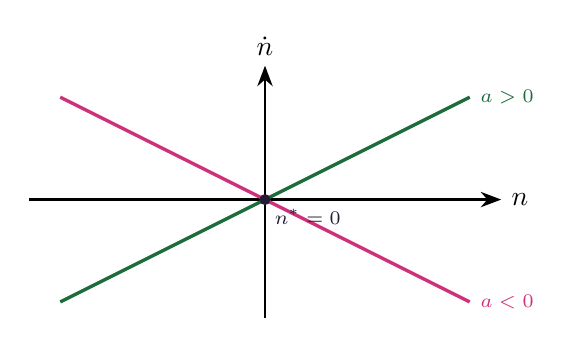
\begin{tikzpicture}[scale=1]
  \draw[->,thick] (-3,0)--(3,0) node[right]{$n$};
  \draw[->,thick] (0,-1.5)--(0,1.7) node[above]{$\dot n$};
  \draw[pgreen,very thick] (-2.6,-1.3)--(2.6,1.3) node[right,font=\scriptsize]{$a>0$};
  \draw[ppink,very thick] (-2.6,1.3)--(2.6,-1.3) node[right,font=\scriptsize]{$a<0$};
  \fill[ink] (0,0) circle (2pt) node[below right,font=\scriptsize]{$n^*=0$};
\end{tikzpicture}
\figcap{The geometric view: plot $\dot n$ against $n$. Where the line is above the axis $n$ grows, and where it is below $n$ shrinks.
For $a<0$ every state flows towards $0$; for $a>0$ every state flows away from $0$.}
\end{center}

The bonus hour asks how the system \emph{behaves around} a fixed point. That question has a name.

\begin{defn}[Converge, diverge]
A solution \term{converges} to $n^*$ if $n(t)\to n^*$ as $t\to\infty$: it gets as close as you like and stays there.
It \term{diverges} if $|n(t)|$ grows without bound.
Example: $n(t)=100e^{-0.1t}$ converges to $0$ ($100\to36.8\to13.5\to\dots$ at $t=0,10,20$);
$n(t)=100e^{0.1t}$ diverges ($100\to272\to739\to\dots$).
\end{defn}

\begin{defn}[Stable and unstable fixed point]
Start the system \emph{near} the fixed point, not exactly on it.
\begin{itemize}
  \item The fixed point is \term{stable} if every such start \hl{converges back} to it.
  \item It is \term{unstable} if some starts arbitrarily close to it \hl{move away} from it.
\end{itemize}
For $\dot n = an$: if $a<0$, $n(t)=n_0e^{at}\to0$ from any $n_0$, so $n^*=0$ is stable. If $a>0$, even $n_0=0.001$ grows like $0.001e^{at}$, so $n^*=0$ is unstable.
\end{defn}

\begin{intuition}[A ball on a landscape]
A stable fixed point is a ball resting at the bottom of a valley: nudge it and it rolls back. An unstable one is a ball balanced on a hilltop:
it is at rest too, but the smallest nudge sends it away. In the plot above, \hl{the line crossing zero going down ($a<0$) means stable; going up ($a>0$) means unstable}.
\end{intuition}

\section{Adding outside input: $\dot n = an + I(t)$}

Now let infected travellers enter the country at a rate $I(t)$ (people per unit time), and take $a<0$. The equation becomes
\[ \dot n(t) = a\,n(t) + I(t). \]

\begin{formula}[Solution with input]
\[ \boxed{\, n(t) = n_0\,e^{at} + \int_0^t I(\tilde t\,)\, e^{a(t-\tilde t\,)}\, d\tilde t \,} \]
\end{formula}

\textbf{Where it comes from (same trick as before)} \src{LMLF 2.A.1}:
\begin{enumerate}
  \item Rewrite: $\dot n - an = I$. Multiply by $e^{-at}$: $\;\frac{d}{dt}\big(n\,e^{-at}\big) = I(t)\,e^{-at}$.
  \item Integrate from $0$ to $t$: $\;n(t)e^{-at} - n_0 = \int_0^t I(\tilde t\,)\,e^{-a\tilde t}\,d\tilde t$.
  \item Multiply by $e^{at}$: $\;n(t) = n_0e^{at} + \int_0^t I(\tilde t\,)\,e^{a(t-\tilde t\,)}\,d\tilde t$.
\end{enumerate}

\begin{intuition}[Reading the formula]
\begin{itemize}
  \item $n_0e^{at}$: the people who were sick at the start, whose number decays (for $a<0$) exactly as before.
  \item $\int_0^t I(\tilde t\,)e^{a(t-\tilde t\,)}d\tilde t$: \hl{every earlier arrival, weighted by how long ago it happened}.
        People who arrived at time $\tilde t$ have had $t-\tilde t$ time to recover (or to spread the illness), so their
        contribution today is $I(\tilde t\,)$ multiplied by $e^{a(t-\tilde t\,)}$.
\end{itemize}
If a big group arrives at some time $t_1$, it shows up as a jump at $t_1$ that then fades with the factor $e^{a(t-t_1)}$.
\end{intuition}

\begin{example}[Constant input: a new balance point]
Take $a=-0.1$/day, a constant $I=5$ people/day, and $n_0=100$. The integral is
$\int_0^t 5\,e^{-0.1(t-\tilde t)}d\tilde t = 50\,(1-e^{-0.1t})$, so
\[ n(t) = 100e^{-0.1t} + 50(1-e^{-0.1t}) = 50 + 50\,e^{-0.1t}. \]
\begin{center}
\begin{tabular}{c|ccccc}
$t$ (days) & 0 & 7 & 14 & 30 & 60\\\hline
$n(t)$ & 100 & 74.8 & 62.3 & 52.5 & 50.1
\end{tabular}
\end{center}
The number settles at $n^* = 50$, which is the fixed point: $\dot n = -0.1\cdot 50 + 5 = 0$. In general a constant input
gives $n^* = -I/a$ \src{LMLF eq.\ 2.64}. Arrivals ($5$/day) exactly balance recoveries ($0.1\times50$/day).
\end{example}

\begin{defn}[Convolution]
An integral of this form is a \term{convolution}:
\[ (f*g)(t) = \int_0^t f(\tilde t\,)\,g(t-\tilde t\,)\,d\tilde t. \]
Our integral is $I * e^{at}$. It sums up the contributions of the input at all past times, each one weighted (``modulated'')
by $e^{at}$ evaluated at how long ago it happened. The limits $[0,t]$ sometimes change (e.g.\ $(-\infty,t]$).
\end{defn}

\section{The link to the rate model}\label{sec:tie}

The rate model of the course has exactly this shape:
\begin{formula}[Rate model with dynamics]
\[ \tau\,\dot r = -r + g(h), \qquad h = Jr + h^{\text{ext}} \]
For a network of $N$ neurons: $\;\tau\dot r_i = -r_i + g\Big(\sum_{j=1}^N J_{ij}r_j + h_i^{\text{ext}}\Big)$.
\end{formula}

Compare it with $\dot n = an + I$ term by term:
\begin{center}
\renewcommand{\arraystretch}{1.25}
\begin{tabular}{>{\columncolor{border}}l l}
\thd{EPIDEMIC} & \cellcolor{border}\thd{RATE MODEL}\\
\rowcolor{surface}\cellcolor{border}\color{surface} $n$ = number sick & $r$ = firing rate\\
\rowcolor{surface2}\cellcolor{border}\color{surface} $a\,n$ with $a<0$ & $-r/\tau$: decay with $a=-1/\tau$\\
\rowcolor{surface}\cellcolor{border}\color{surface} input $I(t)$ & $g(h(t))/\tau$\\
\end{tabular}
\end{center}

\begin{intuition}[Decay towards silence]
The $-r$ term is a decaying exponential. Without stimulation, a neuron's rate \hl{returns to zero on the time scale $\tau$}.
Input through $g(h)$ pushes it up again. The difference from the epidemic is that $h$ depends on $r$ itself (through $J$),
so the ``input'' is fed back by the network. This is what makes network dynamics interesting.
\end{intuition}

\begin{example}[What $\tau$ means, with numbers]
A single neuron with a constant input $h$ switched on at $t=0$, starting from $r(0)=0$. Plugging $a=-1/\tau$ and the
constant input $g(h)/\tau$ into the solution with input gives \src{LMLF eq.\ 2.7}
\[ r(t) = g(h)\big(1-e^{-t/\tau}\big). \]
With $\tau = 10$\,ms (the membrane integration time of \S\ref{sec:scales}):
\begin{center}
\begin{tabular}{c|cccccc}
$t$ (ms) & 0 & 5 & 10 & 20 & 30 & 50\\\hline
$r/g(h)$ & 0 & 0.39 & \hl{0.63} & 0.86 & 0.95 & 0.99
\end{tabular}
\end{center}
\textbf{$\tau$ is the time to reach $1-1/e\approx 63\%$ of the final rate.} The neuron does not respond instantly; it follows its input with a lag of about $\tau$.
\end{example}

\begin{pitfall}[Shorthand]
We usually write $r,\dot r$ for $r(t),\dot r(t)$. Also, $g(h(r(t)))$ looks scary, but in practice the terms are written out explicitly.
\end{pitfall}

% =================================================================
\parttitle{PART C \textperiodcentered\ TA SESSION 1}{Linear Systems: Solving $\dot{\vec x} = M\vec x$}
% =================================================================

\section{Why linear systems?}

The TA session solves the rate model for $N$ neurons in the simplest case, a \hl{linear activation function} $g(h)=h$.
Then (with $\tau=1$ and no external input) the rate equation becomes
\[ \dot r_i = -r_i + \sum_{j} J_{ij} r_j \quad\iff\quad \dot{\vec r} = (J - I)\,\vec r, \]
a system of the form $\dot{\vec x} = M\vec x$ with the matrix $M = J-I$. So we need to know how to solve $\dot{\vec x} = M\vec x$.

\section{From one equation to many}

\textbf{One equation.} $\dot x = ax \Rightarrow x(t) = Ce^{at}$ (Part B).

\textbf{Many separate equations.} $\dot x_i = a_ix_i$ for $i=1,\dots,N$. Each equation contains only its own variable, so we solve each one
separately: $x_i(t) = C_ie^{a_it}$. Easy.

\textbf{Coupled equations.} Now mix the variables:
\[ \dot x_1 = 3x_1 + 2x_2, \qquad \dot x_2 = x_1 - x_2. \]

\begin{defn}[Coupled]
Equations are \term{coupled} when the rate of change of one variable depends on the others. Here $\dot x_1$ depends on
$x_2$ and $\dot x_2$ depends on $x_1$, so neither can be solved alone.
\end{defn}

\begin{intuition}[The plan]
As with high-school simultaneous equations, we want to \hl{rearrange the equations so that each one involves only itself}.
Linear algebra does this: in the basis of the eigenvectors the equations decouple.
\end{intuition}

\textbf{Matrix form.}
\[ \begin{pmatrix}\dot x_1\\ \dot x_2\end{pmatrix} = \underbrace{\begin{pmatrix}3&2\\1&-1\end{pmatrix}}_{M}\begin{pmatrix}x_1\\x_2\end{pmatrix}
\qquad\iff\qquad \dot{\vec x} = M\vec x. \]

\section{Worked example: \texorpdfstring{$M = \left(\begin{smallmatrix}3&2\\1&-1\end{smallmatrix}\right)$}{M = (3 2; 1 -1)}}

\subsection{Step 1: eigenvalues}

\begin{defn}[Eigenvalue, right eigenvector]
$\lambda$ is an \term{eigenvalue} of $M$ with \term{(right) eigenvector} $\vec u\neq 0$ if $M\vec u = \lambda\vec u$:
$M$ only stretches $\vec u$, it does not turn it.
\end{defn}

Solve $\det(M-\lambda I) = 0$:
\[ \det\begin{pmatrix}3-\lambda&2\\1&-1-\lambda\end{pmatrix} = (3-\lambda)(-1-\lambda) - 2 = \lambda^2 - 2\lambda - 5 = 0
\;\Rightarrow\; \lambda = \frac{2\pm\sqrt{4+20}}{2} = 1\pm\sqrt6. \]
\[ \lambda_1 = 1-\sqrt6 \approx \hl{-1.449}, \qquad \lambda_2 = 1+\sqrt6 \approx \hl{+3.449}. \]

\subsection{Step 2: right eigenvectors}

Write $\vec u = (x,1)^\top$. The first row of $M\vec u=\lambda\vec u$ reads $3x + 2 = \lambda x$, so $x = \dfrac{2}{\lambda-3}$.
\begin{itemize}
  \item $\lambda_1 = 1-\sqrt6$: $x = \dfrac{2}{-2-\sqrt6} = \dfrac{2(\sqrt6-2)}{(-2-\sqrt6)(\sqrt6-2)} = \dfrac{2(\sqrt6-2)}{-2} = 2-\sqrt6$.
        So $\vec u_1 = \begin{pmatrix}2-\sqrt6\\1\end{pmatrix}\approx\begin{pmatrix}-0.449\\1\end{pmatrix}$.
  \item $\lambda_2 = 1+\sqrt6$: in the same way, $\vec u_2 = \begin{pmatrix}2+\sqrt6\\1\end{pmatrix}\approx\begin{pmatrix}4.449\\1\end{pmatrix}$.
\end{itemize}

\textbf{Check $\vec u_1$:}
\[ \begin{pmatrix}3&2\\1&-1\end{pmatrix}\begin{pmatrix}2-\sqrt6\\1\end{pmatrix}
= \begin{pmatrix}6-3\sqrt6+2\\ 2-\sqrt6-1\end{pmatrix} = \begin{pmatrix}8-3\sqrt6\\ 1-\sqrt6\end{pmatrix}
= (1-\sqrt6)\begin{pmatrix}2-\sqrt6\\1\end{pmatrix}. \checkmark \]
(Indeed $(1-\sqrt6)(2-\sqrt6) = 2-\sqrt6-2\sqrt6+6 = 8-3\sqrt6$.)

\subsection{Step 3: left eigenvectors}

What if we multiply from the \emph{other} side, using the same vector as a row?
\[ \big(2-\sqrt6,\ 1\big)\begin{pmatrix}3&2\\1&-1\end{pmatrix} = \big(7-3\sqrt6,\ 3-2\sqrt6\big). \]
Is this a multiple of $(2-\sqrt6,\,1)$? It would have to be $(3-2\sqrt6)\cdot(2-\sqrt6,\,1) = (18-7\sqrt6,\ 3-2\sqrt6)$, and the first entries do not match. \textbf{Not an eigenvector from the left.}

\begin{defn}[Left eigenvector]
A row vector $\vec w^\top$ is a \term{left eigenvector} of $M$ if $\vec w^\top M = \lambda\vec w^\top$ (equivalently, $\vec w$ is a right eigenvector of $M^\top$).
Left and right eigenvectors have the \emph{same} eigenvalues, but for a non-symmetric matrix they are \hl{different vectors}.
\end{defn}

Write $\vec w^\top = (y,\,1)$. The first column of $\vec w^\top M = \lambda \vec w^\top$ reads $3y + 1 = \lambda y$, so $y = \dfrac{1}{\lambda-3}$:
\[ \lambda_1:\ \vec w_1^\top = \Big(1-\tfrac{\sqrt6}{2},\ 1\Big)\approx(-0.225,\,1), \qquad
   \lambda_2:\ \vec w_2^\top = \Big(1+\tfrac{\sqrt6}{2},\ 1\Big)\approx(2.225,\,1). \]

\begin{pitfall}[When do left and right eigenvectors coincide?]
For a \textbf{symmetric} matrix ($M^\top = M$), left and right eigenvectors are the same, and the eigenvectors can be chosen
orthogonal (``orthogonally diagonalizable''). The TA notes' footnote gives the more general condition $M^\top M = MM^\top$ (a \emph{normal}
matrix). Our $M$ is not symmetric ($M_{12}=2\neq1=M_{21}$), so its left and right eigenvectors differ. The sentence in the TA
notes ``\dots and the matrix is orthogonal diagonalizable. In this case it isn't'' means: \emph{a symmetric matrix would be orthogonally diagonalizable; this one is not.}
\end{pitfall}

\subsection{Step 4: diagonalize}

Put the right eigenvectors into the columns of $U$ and the eigenvalues on the diagonal of $D$:
\[ U = \begin{pmatrix}2-\sqrt6 & 2+\sqrt6\\ 1 & 1\end{pmatrix},\qquad
   D = \begin{pmatrix}1-\sqrt6 & 0\\ 0 & 1+\sqrt6\end{pmatrix},\qquad
   \boxed{M = U D U^{-1}}. \]
\textbf{The rows of $U^{-1}$ are the left eigenvectors}, each scaled so that $\vec w_k^\top\vec u_k = 1$ \src{LMLF App.\ 2.A.2}. Check:
\[ \vec w_1^\top\vec u_1 = \big(1-\tfrac{\sqrt6}{2}\big)(2-\sqrt6) + 1 = 6-2\sqrt6,\qquad
   \vec w_2^\top\vec u_2 = 6+2\sqrt6,\qquad
   \vec w_1^\top\vec u_2 = \big(1-\tfrac{\sqrt6}{2}\big)(2+\sqrt6)+1 = 0. \]
So
\[ U^{-1} = \begin{pmatrix} \big(1-\tfrac{\sqrt6}{2},\ 1\big)\big/(6-2\sqrt6)\\[3pt] \big(1+\tfrac{\sqrt6}{2},\ 1\big)\big/(6+2\sqrt6)\end{pmatrix}. \]

\begin{intuition}[Why left eigenvectors are useful]
A left eigenvector of one eigenvalue is \hl{perpendicular to the right eigenvectors of all the other eigenvalues}
($\vec w_1^\top\vec u_2 = 0$ above). So taking the dot product with $\vec w_k$ ``filters out'' all components except the $k$-th one.
That is how we read off the coordinates of $\vec x$ in the eigenbasis.
\end{intuition}

\begin{pitfall}[The TA notes' $U^{-1}DU$]
The TA notes write $U^{-1}DU = M$ with the \emph{left}-eigenvector matrix called $U$ and the right-eigenvector matrix
called $U^{-1}$. The order (right eigenvectors, then $D$, then left eigenvectors) is correct, but \textbf{the left eigenvectors
must be divided by $6\mp2\sqrt6$}. Without this scaling the two matrices are not inverses of each other, and the product is not $M$.
In these notes, $U$ always means the matrix of right eigenvectors, as in the book: $M = UDU^{-1}$.
\end{pitfall}

\subsection{Step 5: decouple and solve}

Write $\vec x$ in the eigenbasis: $\vec x(t) = \tilde x_1(t)\,\vec u_1 + \tilde x_2(t)\,\vec u_2$, i.e.\ $\tilde{\vec x} = U^{-1}\vec x$. Then
\[ \dot{\tilde{\vec x}} = U^{-1}\dot{\vec x} = U^{-1}M\vec x = U^{-1}(UDU^{-1})\vec x = D\,\tilde{\vec x}. \]
$D$ is diagonal, so the equations are \hl{decoupled}:
\begin{formula}[Decoupled equations]
\[ \dot{\tilde x}_1 = (1-\sqrt6)\,\tilde x_1 \Rightarrow \tilde x_1(t) = C_1e^{(1-\sqrt6)t},\qquad
   \dot{\tilde x}_2 = (1+\sqrt6)\,\tilde x_2 \Rightarrow \tilde x_2(t) = C_2e^{(1+\sqrt6)t}. \]
\[ \vec x(t) = C_1e^{\lambda_1t}\,\vec u_1 + C_2e^{\lambda_2t}\,\vec u_2,\qquad C_k = \tilde x_k(0) = \frac{\vec w_k^\top\vec x(0)}{\vec w_k^\top\vec u_k}. \]
\end{formula}

\begin{example}[Start at $\vec x(0) = (1,0)$]
\[ C_1 = \frac{1-\sqrt6/2}{6-2\sqrt6} = -\frac{1}{2\sqrt6}\approx-0.204,\qquad C_2 = \frac{1+\sqrt6/2}{6+2\sqrt6} = \frac{1}{2\sqrt6}\approx 0.204. \]
Check at $t=0$: $\frac{1}{2\sqrt6}\big[-(2-\sqrt6,1)+(2+\sqrt6,1)\big] = \frac{1}{2\sqrt6}(2\sqrt6,\,0) = (1,0)$. \checkmark
\[ \vec x(t) = \frac{1}{2\sqrt6}\Big[\,e^{(1+\sqrt6)t}\begin{pmatrix}2+\sqrt6\\1\end{pmatrix} - e^{(1-\sqrt6)t}\begin{pmatrix}2-\sqrt6\\1\end{pmatrix}\Big]. \]
\begin{center}
\renewcommand{\arraystretch}{1.2}
\begin{tabular}{c|cc|cc}
$t$ & $|\tilde x_1| = 0.204\,e^{-1.449t}$ & $\tilde x_2 = 0.204\,e^{3.449t}$ & $x_1(t)$ & $x_2(t)$\\\hline
0 & 0.204 & 0.204 & 1.00 & 0.00\\
0.25 & 0.142 & 0.484 & 2.22 & 0.34\\
0.5 & 0.099 & 1.145 & 5.14 & 1.05\\
1 & 0.048 & 6.43 & 28.6 & 6.38\\
2 & 0.011 & 202 & 900 & 202\\
\end{tabular}
\end{center}
The $\vec u_1$ component \emph{dies out}, while the $\vec u_2$ component \emph{explodes}. After a short while $\vec x(t)$ points almost exactly along
$\vec u_2 = (4.449,1)$: at $t=2$, $x_1/x_2 = 900/202 \approx 4.45$.
\end{example}

\section{Vocabulary: fixed points and stability in two dimensions}

The words from the bonus hour (Part B: fixed point, converge, diverge, stable, unstable) carry over to vectors. Here they are in two dimensions.

\begin{defn}[State, trajectory, phase portrait]
The \term{state} is the vector $\vec x=(x_1,x_2)$, a point in the plane. As time runs, the state moves and traces a curve, the \term{trajectory}.
A \term{phase portrait} is a drawing of many trajectories at once in the $(x_1,x_2)$ plane, with arrows for the direction of motion.
It shows how the system behaves from \emph{every} starting point.
\end{defn}

\begin{defn}[Fixed point of $\dot{\vec x}=M\vec x$]
A \term{fixed point} is a state where $\dot{\vec x}=\vec 0$, i.e.\ $M\vec x^*=\vec 0$. The origin $\vec x^*=\vec0$ is always one.
If $M$ is invertible (no eigenvalue equal to $0$) it is the \emph{only} one. Example: for $M=\begin{pmatrix}3&2\\1&-1\end{pmatrix}$, $\det M=-5\neq0$, so $\vec 0$ is the only fixed point.
\end{defn}

\begin{defn}[Converge, diverge, stable, unstable (vectors)]
\begin{itemize}
  \item The system \term{converges} to $\vec 0$ if $\vec x(t)\to\vec 0$, i.e.\ every component goes to $0$. It \term{diverges} if the length $\norm{\vec x(t)}$ grows without bound.
  \item The fixed point $\vec 0$ is \term{stable} if trajectories that start near it converge to it, and \term{unstable} if some start arbitrarily close to it and move away.
\end{itemize}
\end{defn}

\begin{intuition}[For linear systems, ``near'' does not matter]
If $\vec x(t)$ is a solution of $\dot{\vec x}=M\vec x$, so is $c\,\vec x(t)$ for any number $c$ (multiply both sides by $c$). So a start at
$(0.001,0)$ behaves exactly like a start at $(1,0)$, only scaled down by $1000$. Hence, for linear systems,
\hl{stable $\iff$ converges from every start}, and \hl{unstable $\iff$ diverges from some start}.
\end{intuition}

\begin{example}[Two diagonal systems]
$M=\Diag(-1,-2)$, start $(1,1)$: the equations are already decoupled, $\vec x(t)=(e^{-t},e^{-2t})$. At $t=0,1,2$: $(1,1)$, $(0.37,0.14)$, $(0.14,0.02)$. It converges: $\vec0$ is \textbf{stable}.

$M=\Diag(1,-1)$, start $(1,1)$: $\vec x(t)=(e^{t},e^{-t})$: $(1,1)$, $(2.7,0.37)$, $(7.4,0.14)$. The second component dies but the first explodes: it diverges, so $\vec0$ is \textbf{unstable}.
\end{example}

\begin{defn}[Saddle]
A \term{saddle} is a fixed point that attracts along some directions and repels along others: one eigenvalue negative, one positive.
The name comes from a horse's saddle: from front to back it curves up, from side to side it curves down. A saddle is \textbf{unstable},
since almost every start eventually leaves along the repelling direction. $\Diag(1,-1)$ above is a saddle, and so is our worked example.
\end{defn}

\begin{center}
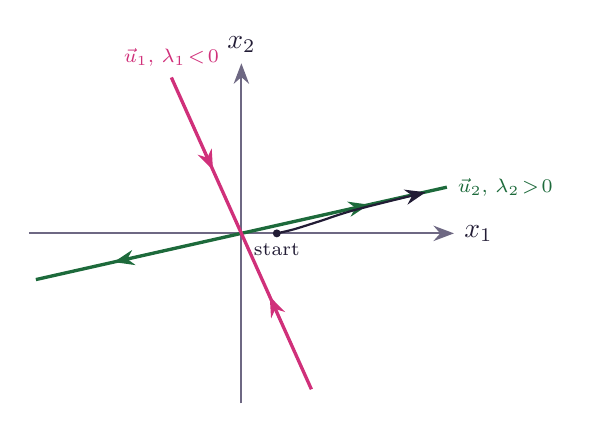
\begin{tikzpicture}[scale=0.9]
  \draw[->,thick,muted] (-3,0)--(3,0) node[right,ink]{$x_1$};
  \draw[->,thick,muted] (0,-2.4)--(0,2.4) node[above,ink]{$x_2$};
  % u2 direction (unstable)
  \draw[pgreen,very thick] (-2.9,-0.652)--(2.9,0.652) node[right,font=\scriptsize]{$\vec u_2$, $\lambda_2\!>\!0$};
  \draw[pgreen,->,thick] (0.9,0.202)--(1.8,0.405); \draw[pgreen,->,thick] (-0.9,-0.202)--(-1.8,-0.405);
  % u1 direction (stable)
  \draw[ppink,very thick] (0.988,-2.2)--(-0.988,2.2) node[above,font=\scriptsize]{$\vec u_1$, $\lambda_1\!<\!0$};
  \draw[ppink,->,thick] (-0.8,1.78)--(-0.4,0.89); \draw[ppink,->,thick] (0.8,-1.78)--(0.4,-0.89);
  % trajectory from (1,0)
  \draw[ink,thick,->] plot[smooth] coordinates {(0.5,0) (0.75,0.06) (1.1,0.17) (1.6,0.33) (2.6,0.58)};
  \fill[ink] (0.5,0) circle (1.6pt) node[below,font=\scriptsize]{start};
\end{tikzpicture}
\figcap{Phase portrait of the example (a \emph{saddle}). Along $\vec u_1$ the state shrinks towards $0$; along $\vec u_2$ it grows. A typical
starting point (black) is first pulled in along $\vec u_1$ and then pushed out along $\vec u_2$.}
\end{center}

\section{What the eigenvalues tell us: stability}

\begin{intuition}[The whole story is in the eigenvalues]
In the standard basis, $x_1$ and $x_2$ are linear combinations of $\tilde x_1$ and $\tilde x_2$, which we already know.
So to know whether the system \emph{converges} or \emph{diverges}, it is enough to look at the \hl{signs of the eigenvalues}; we do not need the eigenvectors.
\end{intuition}

\begin{formula}[Stability of $\dot{\vec x} = M\vec x$]
\begin{itemize}
  \item \textbf{All eigenvalues negative} $\Rightarrow$ every component $e^{\lambda_kt}\to 0$: from \emph{any} start, $\vec x(t)\to\vec 0$. The fixed point $\vec 0$ is \term{stable}.
  \item \textbf{At least one eigenvalue positive} $\Rightarrow$ that component grows like $e^{\lambda t}$: the system \term{diverges} from almost every start.
\end{itemize}
\[ \boxed{\text{converges to } \vec 0 \text{ from every start} \iff \text{all eigenvalues are negative}} \]
(If the eigenvalues are complex numbers, read ``negative'' as ``negative real part'' \src{LMLF App.\ 2.A.2}.)
\end{formula}

\begin{pitfall}[Corrections to the TA notes]
\begin{itemize}
  \item The notes say ``\emph{both of them just increase over time}''. That is not true for this $M$: $\lambda_1 = 1-\sqrt6\approx-1.45$ is \textbf{negative}, so
        $\tilde x_1$ \emph{decays}. The system still diverges, but only because $\lambda_2 > 0$.
  \item The notes say ``\emph{the system diverges if and only if all of the eigenvalues are negative}''. This is a typo. The correct statement is
        \textbf{converges if and only if all eigenvalues are negative}, or equivalently \textbf{diverges if and only if at least one eigenvalue is positive}.
  \item ``Diverges from almost every start'': if you start \emph{exactly} on the line of $\vec u_1$, then $C_2=0$ and you slide into $\vec 0$.
        Any tiny deviation off that line gets amplified.
\end{itemize}
\end{pitfall}

\section{The $2\times2$ shortcut: trace and determinant}

For two neurons we do not even need the eigenvalues themselves. Two facts from linear algebra:
\[ \operatorname{Tr}(M) = \sum_i\lambda_i = \lambda_1+\lambda_2, \qquad \operatorname{Det}(M) = \prod_i\lambda_i = \lambda_1\lambda_2. \]

\textbf{The argument, step by step.}
\begin{enumerate}
  \item If both eigenvalues are negative, then their sum is negative: $\operatorname{Tr}<0$.
  \item If both eigenvalues are negative, then their product is positive (negative $\times$ negative): $\operatorname{Det}>0$.
  \item So if $\operatorname{Tr}\ge 0$ or $\operatorname{Det}\le 0$, the eigenvalues are \emph{not} both negative, and the system does not converge.
  \item Conversely, $\operatorname{Det}>0$ means the two eigenvalues have the same sign (or are complex conjugates with the same real part $\operatorname{Tr}/2$),
        and then $\operatorname{Tr}<0$ makes that sign negative \src{LMLF App.\ 2.A.2}.
\end{enumerate}

\begin{formula}[$2\times2$ stability test]
\[ \dot{\vec x} = M\vec x \text{ converges to } \vec 0 \iff \boxed{\operatorname{Tr}(M) < 0 \ \text{ and } \ \operatorname{Det}(M) > 0} \]
\end{formula}

\begin{example}[Three matrices, no eigenvalues needed]
\begin{center}
\renewcommand{\arraystretch}{1.3}
\begin{tabular}{>{\columncolor{border}}c c c L{6.2cm}}
\thd{$M$} & \cellcolor{border}\thd{TR} & \cellcolor{border}\thd{DET} & \cellcolor{border}\thd{VERDICT}\\
\rowcolor{surface} \cellcolor{border}\color{surface}$\begin{pmatrix}3&2\\1&-1\end{pmatrix}$ & $2$ & $-3-2=-5$ & Det $<0$: one positive, one negative eigenvalue $\Rightarrow$ diverges\\
\rowcolor{surface2} \cellcolor{border}\color{surface}$\begin{pmatrix}-1&0\\0&-2\end{pmatrix}$ & $-3$ & $2$ & Tr $<0$, Det $>0$ $\Rightarrow$ converges\\
\rowcolor{surface} \cellcolor{border}\color{surface}$\begin{pmatrix}-2&3\\1&-1\end{pmatrix}$ & $-3$ & $2-3=-1$ & Det $<0$ $\Rightarrow$ diverges, \emph{even though} Tr $<0$\\
\end{tabular}
\end{center}
For the first one: $\lambda_1+\lambda_2 = (1-\sqrt6)+(1+\sqrt6) = 2$ and $\lambda_1\lambda_2 = 1-6 = -5$, matching Tr and Det. \checkmark
\end{example}

\begin{pitfall}[A negative trace is not enough]
The third matrix shows why we need \emph{both} conditions: its eigenvalues are $\frac{-3\pm\sqrt{13}}{2}\approx 0.30$ and $-3.30$.
They sum to a negative number, but one of them is positive.
\end{pitfall}

\begin{plainbox}
\textbf{Further reading from the TA notes:} Appendix 2.A.2 of the book \src{LMLF} gives the same derivation for $N$ dimensions:
diagonalize $M = UDU^{-1}$, decouple into $\dot{\tilde x}_k = \mu_k\tilde x_k$, and the dynamics converge to $0$ if all the $\mu_k$ are negative (real part).
\end{plainbox}

% =================================================================
\parttitle{WEEK 01}{Practice Problems and Summary}
% =================================================================

\section{Practice problems with full solutions}

\begin{example}[P1: Rate model]
Two neurons with threshold-linear $g$: $J = \begin{pmatrix}0 & -1\\ 2 & 0\end{pmatrix}$, $b = (3,\,1)$, current rates $r=(2,\,4)$.
Compute $g(\sum_jJ_{ij}r_j+b_i)$ for both neurons. Which neuron is inhibitory, by Dale's principle?

\textbf{Solution.} $h_1 = 0\cdot2 + (-1)\cdot4 + 3 = -1 \Rightarrow g = 0$. \quad $h_2 = 2\cdot2 + 0\cdot4 + 1 = 5 \Rightarrow g = 5$.
The synapses \emph{from} neuron 2 are column 2 of $J$: $J_{12}=-1<0$, so neuron 2 is inhibitory. Column 1 has $J_{21}=2>0$, so neuron 1 is excitatory.
\end{example}

\begin{example}[P2: Solving $\dot n = an$]
A population of bacteria obeys $\dot n = 0.3\,n$ (per hour) with $n(0)=1000$. When does it reach $8000$?

\textbf{Solution.} $n(t) = 1000e^{0.3t} = 8000 \Rightarrow e^{0.3t}=8 \Rightarrow t = \ln 8/0.3 = 3\ln2/0.3 \approx 6.93$\,h.
Equivalently, it doubles every $\ln2/0.3\approx 2.31$\,h, and $8 = 2^3$ means three doublings.
\end{example}

\begin{example}[P3: Fixed point with input]
$\dot n = -0.5\,n + 4$, $n(0)=0$. Find the fixed point and $n(t)$.

\textbf{Solution.} Fixed point: $0 = -0.5n^*+4 \Rightarrow n^*=8$. Using the solution with input (with $a=-0.5$, $I=4$, $n_0=0$):
$n(t) = \int_0^t 4e^{-0.5(t-\tilde t)}d\tilde t = 8(1-e^{-0.5t})$. Check: $n(0)=0$, $n(\infty)=8$, and $\dot n = 4e^{-0.5t} = -0.5\cdot 8(1-e^{-0.5t}) + 4$. \checkmark
\end{example}

\begin{example}[P4: Time constant]
A neuron with $\tau = 20$\,ms receives a constant input from $t=0$, with $g(h) = 50$\,Hz and $r(0)=0$. What is $r$ at $t=20$\,ms and $t=60$\,ms?

\textbf{Solution.} $r(t) = 50(1-e^{-t/20})$. $r(20) = 50(1-e^{-1}) \approx 31.6$\,Hz (63\%). $r(60) = 50(1-e^{-3})\approx 47.5$\,Hz (95\%).
\end{example}

\begin{example}[P5: Decoupled solution]
$\dot{\vec x} = M\vec x$ with $M = \begin{pmatrix}-1 & 2\\ 0 & -3\end{pmatrix}$. Find the eigenvalues and eigenvectors, and decide on stability (a) from the eigenvalues and (b) from Tr/Det.

\textbf{Solution.} $M$ is triangular, so the eigenvalues are its diagonal entries: $\lambda_1=-1$, $\lambda_2=-3$.
$\lambda_1=-1$: $(M+I)\vec u = 0 \Rightarrow \begin{pmatrix}0&2\\0&-2\end{pmatrix}\vec u=0 \Rightarrow \vec u_1 = (1,0)$.
$\lambda_2=-3$: $(M+3I)\vec u=0 \Rightarrow \begin{pmatrix}2&2\\0&0\end{pmatrix}\vec u = 0\Rightarrow \vec u_2 = (1,-1)$.
So $\vec x(t) = C_1e^{-t}(1,0) + C_2e^{-3t}(1,-1)$.
(a) Both eigenvalues are negative $\Rightarrow$ converges to $\vec 0$. (b) Tr $=-4<0$, Det $=3>0$ $\Rightarrow$ converges. \checkmark
\end{example}

\begin{example}[P6: Tr/Det only]
For which values of $w$ does $\dot{\vec x} = \begin{pmatrix}-1 & w\\ w & -1\end{pmatrix}\vec x$ converge to $\vec 0$?

\textbf{Solution.} Tr $=-2<0$ always. Det $=1-w^2>0 \iff |w|<1$. So it converges exactly when $|w|<1$.
(Check with $w=2$: the eigenvalues are $-1\pm2$, i.e.\ $1$ and $-3$; one is positive $\Rightarrow$ diverges.)
\end{example}

\section{Cheat sheet}

\begin{formula}[Week 01 on one page]
\begin{itemize}
  \item \textbf{Neuron}: soma (cell body), axon (output), dendrites (input). Rest $\approx-70$\,mV, threshold $\approx-50$\,mV.
  \item \textbf{Spike}: $\sim$1\,ms, stereotyped, all-or-none. Spikes are the currency of communication; their shape carries no information.
  \item \textbf{Chemical synapse}: spike $\to$ neurotransmitter $\to$ receptors $\to$ ion channels. Excitatory = depolarize, inhibitory = hyperpolarize.
  \item \textbf{Dale}: all outgoing synapses of a neuron have one sign (one column of $J$).
  \item \textbf{Rate model}: $r_i = g\big(\sum_jJ_{ij}r_j + b_i\big)$, $J_{ij}$ = from $j$ to $i$; with dynamics $\tau\dot r_i = -r_i + g(\cdot)$.
  \item \textbf{Scales}: 1\,nm (molecules) to 1\,m (CNS); 1\,ms (spike) to $10^9$\,s (long-term memory). Human: $10^{11}$ neurons, $10^{14}$--$10^{15}$ synapses.
  \item $\dot n = an \Rightarrow n(t)=n_0e^{at}$; grows if $a>0$, decays if $a<0$; doubling/halving time $\ln2/|a|$.
  \item $\dot n = an + I(t)\Rightarrow n(t) = n_0e^{at} + \int_0^tI(\tilde t)e^{a(t-\tilde t)}d\tilde t$ (a convolution $I*e^{at}$); constant $I$, $a<0$: $n\to -I/a$.
  \item \textbf{Fixed point}: $\dot x = 0$. \quad $\tau$ = time to reach 63\% of the final value.
  \item $\dot{\vec x} = M\vec x$, $M = UDU^{-1}$ ($U$: right eigenvectors as columns; $U^{-1}$: left eigenvectors as rows, scaled so $\vec w_k^\top\vec u_k = 1$).
        $\Rightarrow \vec x(t) = \sum_k C_ke^{\lambda_kt}\vec u_k$.
  \item \textbf{Stable} $\iff$ all $\lambda_k<0$. \textbf{$2\times2$}: stable $\iff$ Tr $<0$ and Det $>0$.
\end{itemize}
\end{formula}

\end{document}
